\documentclass[conference]{IEEEtran}
\IEEEoverridecommandlockouts

% Load biblatex package with IEEE style
\usepackage[backend=biber,style=ieee,citestyle=numeric]{biblatex}
\addbibresource{references.bib}
% The preceding line is only needed to identify funding in preoccupied footnote. If that is unneeded, please comment it out.
% \usepackage{cite} % Commented out as we're using biblatex instead
\usepackage{amsmath,amssymb,amsfonts}
\usepackage{algorithmic}
\usepackage{graphicx}
\usepackage{textcomp}
\usepackage{xcolor}
\usepackage{booktabs}
\usepackage{multirow}
\usepackage{subfigure}
\usepackage{url}
\usepackage{makecell}
\usepackage{threeparttable}
% Use IEEE's default fonts to avoid font warnings
% \usepackage[UTF8, scheme=plain]{ctex} % Ctex package commented out as it's for Chinese typesetting


\def\BibTeX{{\rm B\kern-.05em{\sc i\kern-.025em b}\kern-.08em
    T\kern-.1667em\lower.7ex\hbox{E}\kern-.125emX}}

\begin{document}
\sloppy

\title{GRCR-Net: A Complex Residual Network with GPR Denoising and Rotational Augmentation for Automatic Modulation Classification}

\author{
% \IEEEauthorblockN{1\textsuperscript{st} Junkai Li*}
\IEEEauthorblockN{Junkai Li*}
\IEEEauthorblockA{
\textit{College of Information Engineering} \\
\textit{Zhejiang University of Technology}\\
Hangzhou, China\\
302023568066@zjut.edu.cn}
}

\maketitle

\begin{abstract}
Automatic Modulation Classification (AMC) is a key technology in intelligent wireless communications, crucial for enhancing spectral efficiency and network performance.
However, existing deep learning methods suffer from a significant degradation in classification accuracy under low Signal-to-Noise Ratio (SNR) conditions.
This paper addresses this issue by proposing an AMC method.
This method uniquely integrates three core techniques:
First, adaptive Gaussian Process Regression (GPR) is employed for signal denoising, achieving optimal denoising effects at different noise levels through an SNR-adaptive length-scale adjustment strategy.
Second, rotational data augmentation is utilized based on the geometric symmetry of modulation signal constellation diagrams to enrich the training data.
Finally, a hybrid complex convolutional-residual network architecture is designed.
This architecture combines the advantages of Complex Convolutional Networks (ComplexCNN) in processing complex I/Q signals and preserving phase information with the characteristics of Residual Networks (ResNet) in deep feature learning and gradient stability.
Experimental results on the RML2016.10a dataset show that the proposed method achieves a classification accuracy of 65.38\%, significantly outperforming current state-of-the-art methods.
This research provides a robust solution for modulation recognition in complex electromagnetic environments and is of great significance for the development of cognitive radio and next-generation intelligent communication systems.
The code is open-sourced at: \url{https://github.com/LJK666666666/radioML-v3}
\end{abstract}

\begin{IEEEkeywords}
Automatic Modulation Classification, Deep Learning, Complex Neural Networks, ResNet, Gaussian Process Regression, Signal~Denoising, Data~Augmentation
\end{IEEEkeywords}

\section{Introduction}
Automatic Modulation Classification (AMC) is a key technology in modern wireless communication systems, used to identify the modulation scheme of a received signal without prior knowledge. This capability is crucial in applications such as cognitive radio, spectrum monitoring, and military communications, which require receivers to dynamically adapt to various signal types~\cite{dobre2007survey}.

The main challenge of AMC lies in accurately classifying modulation types under low Signal-to-Noise Ratio (SNR), interference, and varying channel conditions. Traditional methods are divided into likelihood-based (LB) and feature-based (FB) categories. Likelihood-based methods (such as maximum likelihood) are theoretically optimal but are computationally complex and require precise knowledge of channel parameters~\cite{hameed2009likelihood}. Feature-based methods classify signals by extracting features and using classifiers like Support Vector Machines (SVMs) or decision trees~\cite{hazza2013overview}. However, these methods rely on expert-designed features and are difficult to generalize across different scenarios.

In recent years, deep learning has become a powerful tool for AMC due to its ability to automatically learn hierarchical features. Convolutional Neural Networks (CNNs) have been particularly successful in this field, with early studies showing their superior performance over traditional methods~\cite{oshea2016convolutional}. Subsequent research has explored deeper architectures, such as ResNet and DenseNet, as well as Long Short-Term Memory (LSTM) networks, to capture the spatial and temporal features of signals~\cite{west2017deep,rajendran2018deep}.

Despite these advancements, AMC in low SNR environments remains challenging, as noise significantly degrades signal quality. To address this, researchers have proposed various strategies, including complex neural networks that directly process I/Q signals to preserve phase information~\cite{xu2025ldcvnn}, and the introduction of attention mechanisms to focus on critical parts of the signal~\cite{ma2023hfecnetca}. Furthermore, data augmentation techniques have been used to improve model generalization, especially for modulation types with inherent symmetries~\cite{zhang2023efficient}.

This paper proposes an enhanced AMC method that integrates a hybrid ComplexCNN-ResNet architecture, Gaussian Process Regression (GPR) adaptive denoising, and rotation-based data augmentation. Our approach aims to leverage the benefits of residual learning and complex signal processing, while mitigating noise effects through adaptive denoising, thereby achieving state-of-the-art classification accuracy on the RML2016.10a dataset, particularly under low SNR conditions.

\section{Related Work}

Automatic Modulation Classification (AMC) has made significant progress in recent years, evolving from traditional feature-based methods to modern deep learning-based approaches. Traditional feature-based methods involve extracting handcrafted features such as higher-order statistics, cyclostationary features, or wavelet transforms, followed by classification using machine learning algorithms~\cite{hazza2013overview}. These methods require expert knowledge for feature design and have limited generalization capabilities under different channel conditions.

With the rise of deep learning, data-driven approaches have significantly improved AMC performance. O'Shea et al.~\cite{oshea2016convolutional} first introduced Convolutional Neural Networks (CNNs) to AMC, demonstrating superior performance over traditional methods on the RML2016.10a dataset. Subsequent studies explored deeper architectures, such as Residual Networks (ResNets) and Densely Connected Networks (DenseNets), to facilitate the training of deeper networks and enhance feature reuse~\cite{west2017deep, patil2021automatic}. Recurrent Neural Networks (RNNs), particularly Long Short-Term Memory (LSTM) networks, have also been employed to capture the temporal dependencies in signal sequences, both on their own and in hybrid architectures combining CNNs and RNNs~\cite{rajendran2018deep, xu2020spatiotemporal}.

To better handle the complex nature of I/Q signals, complex-valued neural networks (CVNNs) have been developed. These networks process complex inputs directly, preserving the critical phase information necessary for distinguishing different modulation types. For instance, Xu et al. proposed LDCVNN~\cite{xu2025ldcvnn}, a lightweight dual-branch CVNN that captures phase information and complex-scaling-equivariant representations, showcasing the potential of this approach for efficient AMC.

Attention mechanisms have also been introduced into AMC models to focus on more informative parts of the signal. Ma et al. proposed HFECNET-CA~\cite{ma2023hfecnetca}, an efficient and lightweight model combining a hybrid feature extraction CNN with a channel attention mechanism (SE block) to achieve a good balance between accuracy and model size. The demand for lightweight models for resource-constrained devices has driven research into highly efficient architectures. Techniques include using separable convolutions, dual-branch complex-valued networks, and hybrid feature extraction, which have resulted in models with fewer than 50K parameters while maintaining high accuracy~\cite{guo2024ulcnn, ma2023hfecnetca, xu2025ldcvnn}.

Transformer models, initially successful in natural language processing, are increasingly applied to AMC due to their ability to model long-range dependencies. Ning et al. introduced AbFTNet~\cite{ning2024abftnet}, an efficient Transformer network for multimodal AMC that processes I/Q and Fractional Fourier Transform (FRFT) data. Its "align before fusion" strategy, employing contrastive learning and an efficient cross-modal aggregation promoting (CAP) module, yielded 64.59\% accuracy on RML2016.10a. This work represents a significant advancement in multimodal AMC by addressing information asynchrony and intensity differences between modalities, establishing a strong benchmark for previous state-of-the-art in this specific sub-domain. 

To improve classification in low-SNR environments, Zhang et al. proposed AMC-Net~\cite{zhang2023amcnet}, a network featuring specialized modules for signal denoising and multi-scale feature extraction. The architecture consists of an Adaptive Correction Module (ACM) that learns to correct the signal's spectrum in the frequency domain, a Multi-Scale Module (MSM) that uses parallel convolutions with varying kernel sizes to capture features at different scales, and a Feature Fusion Module (FFM) based on a self-attention mechanism to effectively learn temporal correlations. On the RML2016.10a dataset, AMC-Net achieved an overall accuracy of 62.51\%, demonstrating strong performance particularly in low SNR conditions. The work highlights the significant impact of its frequency-domain denoising approach on classification accuracy.

Despite these advancements, AMC under low SNR conditions remains challenging. To address this, some methods have incorporated denoising techniques or designed noise-robust architectures~\cite{yao2019modulation}. Data augmentation is another strategy to improve model generalization, with techniques like rotation, flipping, and adding Gaussian noise being applied to simulate various channel conditions and enhance model robustness~\cite{zhang2023efficient}.

In this context, our proposed method integrates a hybrid ComplexCNN-ResNet architecture, Gaussian Process Regression (GPR) adaptive denoising, and rotation-based data augmentation. By combining these elements, we aim to achieve superior AMC performance, particularly under challenging noise conditions, building upon the insights from these diverse research directions.




% \section{Introduction}
% Automatic Modulation Classification (AMC) is a key technology in modern wireless communication systems, used to identify the modulation scheme of a received signal without prior knowledge. This capability is crucial in applications such as cognitive radio, spectrum monitoring, and military communications, which require receivers to dynamically adapt to various signal types~\cite{dobre2007survey}.

% The main challenge of AMC lies in accurately classifying modulation types under low Signal-to-Noise Ratio (SNR), interference, and varying channel conditions. Traditional methods are broadly divided into likelihood-based (LB) and feature-based (FB) categories. Likelihood-based methods (such as maximum likelihood) are theoretically optimal but are computationally complex and require precise knowledge of channel parameters~\cite{hameed2009likelihood}. Feature-based methods, evolving from traditional approaches, classify signals by extracting handcrafted features such as higher-order statistics, cyclostationary features, or wavelet transforms, followed by classification using machine learning algorithms like Support Vector Machines (SVMs) or decision trees~\cite{hazza2013overview}. However, these methods rely on expert knowledge for feature design and possess limited generalization capabilities across different scenarios and channel conditions.

% With the rise of deep learning, data-driven approaches have become a powerful tool for AMC due to their ability to automatically learn hierarchical features, significantly improving performance over traditional methods. O'Shea et al.~\cite{oshea2016convolutional} first introduced Convolutional Neural Networks (CNNs) to AMC, demonstrating their superiority. Subsequent research has explored deeper architectures, such as Residual Networks (ResNets) and Densely Connected Networks (DenseNets), to facilitate the training of deeper networks and enhance feature reuse~\cite{west2017deep, patil2021automatic}. Recurrent Neural Networks (RNNs), particularly Long Short-Term Memory (LSTM) networks, have also been employed to capture the temporal dependencies in signal sequences, both on their own and in hybrid architectures combining CNNs and RNNs~\cite{rajendran2018deep, xu2020spatiotemporal}. 
% % Further DL Architectures
% To better handle the complex nature of I/Q signals and preserve critical phase information, complex-valued neural networks (CVNNs) which process complex inputs directly have been developed, such as the lightweight dual-branch LDCVNN~\cite{xu2025ldcvnn}. Attention mechanisms have also been introduced to focus models on more informative parts of the signal; for instance, HFECNET-CA~\cite{ma2023hfecnetca} combines a hybrid feature extraction CNN with a channel attention mechanism for efficiency. This also reflects a demand for lightweight models for resource-constrained devices, using techniques like separable convolutions~\cite{guo2024ulcnn, ma2023hfecnetca, xu2025ldcvnn}. More recently, Transformer models, known for modelling long-range dependencies, are increasingly applied, such as the multimodal AbFTNet~\cite{ning2024abftnet} which processes both I/Q and Fractional Fourier Transform (FRFT) data.

% % Focus on Low SNR challenge
% Despite these architectural advancements, AMC in low SNR environments remains particularly challenging, as noise significantly degrades signal quality. To address this, researchers have proposed various strategies. Some methods incorporate denoising techniques or design noise-robust architectures~\cite{yao2019modulation}. For instance, AMC-Net~\cite{zhang2023amcnet} proposed an Adaptive Correction Module (ACM) for frequency-domain signal correction, a Multi-Scale Module (MSM), and a self-attention based Feature Fusion Module (FFM), demonstrating the impact of denoising on classification accuracy, particularly in low SNR conditions. Data augmentation is another key strategy used to improve model generalization and robustness by simulating various channel conditions or addressing modulation types with inherent symmetries, using techniques such as rotation, flipping, and adding Gaussian noise~\cite{zhang2023efficient}.

% % Contribution
% In this context, this paper proposes an enhanced AMC method that integrates a hybrid ComplexCNN-ResNet architecture, Gaussian Process Regression (GPR) adaptive denoising, and rotation-based data augmentation. Our approach aims to build upon previous insights by leveraging the benefits of residual learning and complex signal processing, while explicitly mitigating noise effects through adaptive denoising and enhancing robustness via data augmentation, thereby achieving state-of-the-art classification accuracy on the RML2016.10a dataset, particularly under challenging low SNR conditions.





\section{Methodology}

\subsection{Signal Mathematical Model}

In wireless communication systems, modulated signals can be described using a complex baseband representation. Let the original baseband signal be $s(t)$, its complex representation is:

\begin{equation}
s(t) = s_I(t) + js_Q(t)
\end{equation}

where $s_I(t)$ and $s_Q(t)$ represent the In-phase and Quadrature components, respectively, and $j$ is the imaginary unit.

For digital modulated signals, the discrete-time complex baseband signal can be represented as:

\begin{equation}
s[n] = s_I[n] + js_Q[n], \quad n = 0, 1, 2, ..., N-1
\end{equation}

where $N$ is the length of the signal samples. In a practical transmission environment, the received signal is affected by noise, and the received signal model is:

\begin{equation}
r[n] = s[n] + w[n]
\end{equation}

where $w[n]$ represents the noise component. The Signal-to-Noise Ratio (SNR) is defined as the ratio of signal power to noise power:

\begin{equation}
\mathrm{SNR} = 10\log_{10}\left(\frac{P_s}{P_w}\right) \quad(\mathrm{dB})
\end{equation}

The RML2016.10a dataset contains 11 different modulation types, with signal samples generated for each modulation type under different SNR conditions (-20dB to +18dB, in 2dB steps). Each signal sample consists of 128 complex sample points, represented as a real-valued vector of length 256: $[s_I[0], s_Q[0], s_I[1], s_Q[1], ..., s_I[127], s_Q[127]]$.

\begin{figure*}[htbp]
\centering
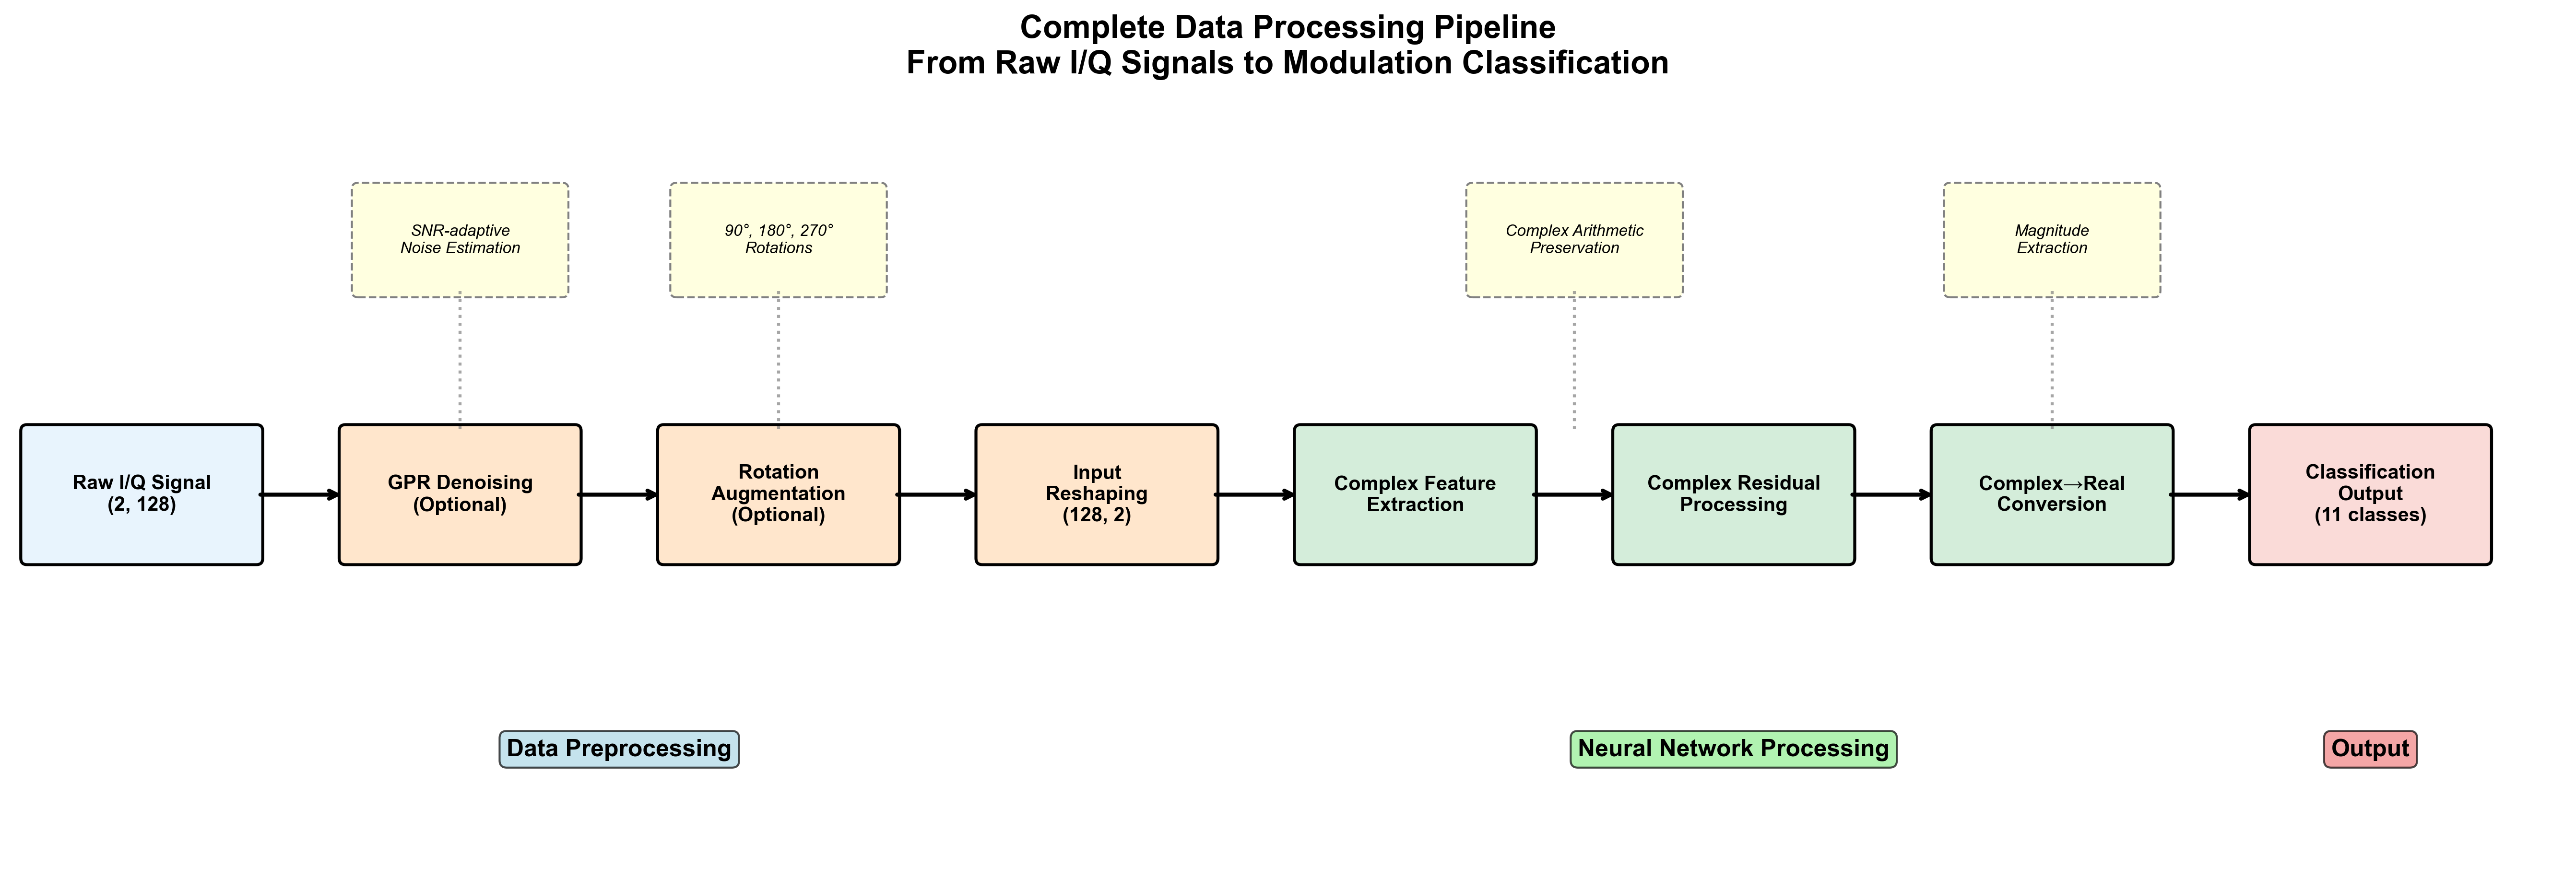
\includegraphics[width=0.9\textwidth]{figure/data_processing_pipeline.png}
\caption{Complete data processing pipeline. This figure illustrates the entire workflow from raw I/Q signal input to final classification output, including GPR denoising, rotational data augmentation, and complex convolutional residual network processing stages.}
\label{fig:data_pipeline}
\end{figure*}

\subsection{Dataset and Preprocessing}

This study utilizes the public RML2016.10a dataset for the automatic modulation classification task. The dataset includes 11 common digital and analog modulation types (8PSK, AM-DSB, AM-SSB, BPSK, CPFSK, GFSK, PAM4, QAM16, QAM64, QPSK, WBFM). For each modulation type, signal samples are generated across a Signal-to-Noise Ratio (SNR) range of -20dB to +18dB in 2dB steps, covering a total of 20 different SNR levels. Each signal sample consists of 128 complex I/Q sample points, stored in the dataset as a real-valued vector of length 256.

The data preprocessing pipeline follows standard machine learning data handling practices. The raw dataset is stored in a structured format, where each sample is associated with its corresponding modulation type and SNR value. The dataset is split using a stratified sampling strategy to ensure a uniform distribution of modulation types and SNR conditions across the training, validation, and test sets. The specific split ratio is: 72\% for the training set, 8\% for the validation set, and the remaining 20\% for the test set.

% During the data preprocessing stage, a flexible SNR filtering mechanism was implemented, allowing for specialized experimental analysis for specific SNR ranges. All class labels were converted to one-hot encoding format to suit the requirements of multi-class classification tasks. To accommodate the input requirements of different neural network architectures, the data supports various tensor format reorganizations: for complex convolutional neural networks, the data is reshaped into a three-dimensional tensor format $(N, 2, L)$, where $N$ is the number of samples, 2 represents the I and Q channels, and $L$ is the sequence length; for traditional convolutional networks, it remains in a two-dimensional matrix format $(N, 2L)$ vector form.



\subsection{Gaussian Process Regression Denoising}

To enhance the model's classification performance under low Signal-to-Noise Ratio (SNR) conditions, this study introduces an adaptive denoising method based on Gaussian Process Regression (GPR). In practical wireless communication systems, received signals are often corrupted by Additive White Gaussian Noise (AWGN), where $w[n] \sim \mathcal{CN}(0, \sigma_n^2)$ represents complex Gaussian white noise with variance $\sigma_n^2$. GPR, as a non-parametric Bayesian method, can effectively model the underlying structure of the signal and suppress such AWGN interference.

The key to GPR denoising lies in the accurate estimation of the noise level, which is achieved through the $\alpha$ parameter (i.e., per-component noise variance $\sigma_n^2$) in the GPR model. For a received noisy signal $r[n]=r_I[n]+jr_Q[n]$, its average power is defined as $P_r = \mathbb{E}[|r[n]|^2]$. In practice, if there are $M$ discrete-time samples, this average power is estimated by summing the instantaneous power $(r_I[k]^2 + r_Q[k]^2)$ of these received signal samples $r[k]$ (where $k=0, \ldots, M-1$) and averaging:
\begin{equation}
P_r = \frac{1}{M}\sum_{k=0}^{M-1}(r_I[k]^2+r_Q[k]^2)
\end{equation}

Assume the power of the original noise-free signal $s[n]$ is $P_s = \mathbb{E}[|s[n]|^2]$, and the power of the noise $w[n]$ is $P_w = \mathbb{E}[|w[n]|^2]$. If the signal and noise are uncorrelated, the total average power of the received signal is:
\begin{equation}
P_r = P_s + P_w
\end{equation}

The Signal-to-Noise Ratio (SNR) is defined as the ratio of the original signal power to the noise power. Its linear value is $\mathrm{SNR}_{\text{linear}} = P_s/P_w$, and the corresponding decibel (dB) value is $\mathrm{SNR}_{\text{dB}} = 10\log_{10}(\mathrm{SNR}_{\text{linear}})$.
Using this definition, we get $P_s = \mathrm{SNR}_{\text{linear}} \cdot P_w$. Substituting this into the total power relation, we have $P_r = \mathrm{SNR}_{\text{linear}} \cdot P_w + P_w = P_w(\mathrm{SNR}_{\text{linear}} + 1)$.
Therefore, the noise power can be calculated from the measured signal power $P_r$ and the given SNR:
\begin{equation}
P_w = \frac{P_r}{\mathrm{SNR}_{\text{linear}} + 1} = \frac{P_r}{10^{\mathrm{SNR}_{\text{dB}}/10} + 1}
\end{equation}
For complex Gaussian white noise $w[n]=w_I[n]+jw_Q[n]$, where the in-phase component $w_I[n]$ and quadrature component $w_Q[n]$ are independent and both follow a zero-mean normal distribution with variance $\sigma_n^2$, i.e., $w_I[n],w_Q[n]\sim\mathcal{N}(0,\sigma_n^2)$. Its total noise power is defined as:
\begin{equation}
P_w=\mathbb{E}[|w[n]|^2]
=\mathbb{E}[w_I[n]^2]+\mathbb{E}[w_Q[n]^2]
=2\sigma_n^2
\end{equation}
From this, the noise variance of a single component can be obtained:
\begin{equation}
\sigma_n^2=\frac{P_w}{2}
\end{equation}
The noise standard deviation is:
\begin{equation}
\sigma_n=\sqrt{\frac{P_w}{2}}
\end{equation}
Combining with equation (6) $P_w=\frac{P_r}{10^{\mathrm{SNR}_{\mathrm{dB}}/10}+1}$, we can further obtain:
\begin{equation}
\sigma_n=\sqrt{\frac{P_r}{2\bigl(10^{\mathrm{SNR}_{\mathrm{dB}}/10}+1\bigr)}}
\end{equation}
\label{eq:sigma_n_calc}
This $\sigma_n^2$ is the noise level parameter $\alpha$ set in the GPR model.

The model uses Radial Basis Function (RBF), Matern, and Rational Quadratic kernel functions to describe the smoothness characteristics of the signal. During the denoising process, the discrete time indices $X=[0,1,\ldots,127]$ are used as input, and the in-phase or quadrature components themselves are the observation targets. Noise suppression is achieved by adding the noise parameter $\alpha=\sigma_n^2$ to the covariance matrix.

To adapt to the signal smoothing requirements under different SNR conditions, this study designed an SNR-based adaptive length-scale strategy. In Gaussian Process Regression, the length-scale parameter $L$ controls the correlation range of the kernel function, directly affecting the strength of the denoising effect. For the RBF kernel function, its expression is:
\begin{equation}
k(x_i, x_j) = \sigma_f^2 \exp\left(-\frac{(x_i - x_j)^2}{2L^2}\right)
\end{equation}
where $\sigma_f^2$ is the signal variance and $L$ is the length-scale parameter. A larger $L$ value means that data points farther apart still have a strong correlation, resulting in a stronger smoothing effect; while a smaller $L$ value makes the smoothing effect more localized, allowing more signal details to be preserved.

Under low SNR conditions, the noise amplitude is relatively large. If an excessively large length-scale $L$ is used at this time, it will lead to the following problems:

\textbf{(1) Oversmoothing of signal features:} When $L$ is too large, GPR will treat signal samples that are far apart as strongly correlated, causing rapid changes in the true signal (such as amplitude and phase jumps in modulated signals) to be mistaken for noise and smoothed out. This oversmoothing can blur the characteristic differences between different modulation types.

\textbf{(2) Loss of time-domain details:} Digital modulated signals contain important time-domain features, such as symbol transition points and instantaneous frequency changes. An excessively large $L$ will cause these detailed features to be smoothed out, reducing the ability of the subsequent classification network to extract effective features.

\textbf{(3) Loss of phase information:} For phase-modulated signals (such as PSK, QAM), rapid changes in phase are key identification features. Oversmoothing will lead to the loss of phase information, severely affecting classification accuracy.

Based on the above analysis, this study proposes an adaptive length-scale strategy: let the base length-scale be $L_0$. When $\mathrm{SNR}\ge0$ dB, take $L=L_0$; when $\mathrm{SNR}<0$ dB, dynamically adjust as follows:
\begin{equation}
L = \max\bigl(L_{\min},\,L_0\bigl(1+\mathrm{SNR}/20\bigr)\bigr)
\end{equation}
where $L_{\min}$ is a preset minimum scale. The core idea of this strategy is: as the SNR decreases, gradually reduce the length-scale $L$, thereby weakening the smoothing effect, and maximizing the preservation of effective signal information while removing noise.

Specifically, when $\mathrm{SNR}=-20$ dB, the length-scale is adjusted to $L=\max(L_{\min}, L_0 \times 0)=L_{\min}$. At this time, the smoothing effect is weakest, prioritizing the preservation of signal details; as the SNR gradually increases, the length-scale increases accordingly, and the smoothing effect is enhanced. This adaptive mechanism ensures sufficient denoising effect in high SNR scenarios, while in low SNR scenarios, it preserves more useful signal features by weakening the smoothing strength, achieving an optimal balance between denoising performance and signal fidelity.

The denoised in-phase and quadrature components are reconstructed into a complex signal, which serves as input data for subsequent neural network training.

\subsection{Rotation-based Data Augmentation}

\begin{figure}[htbp]
\centering
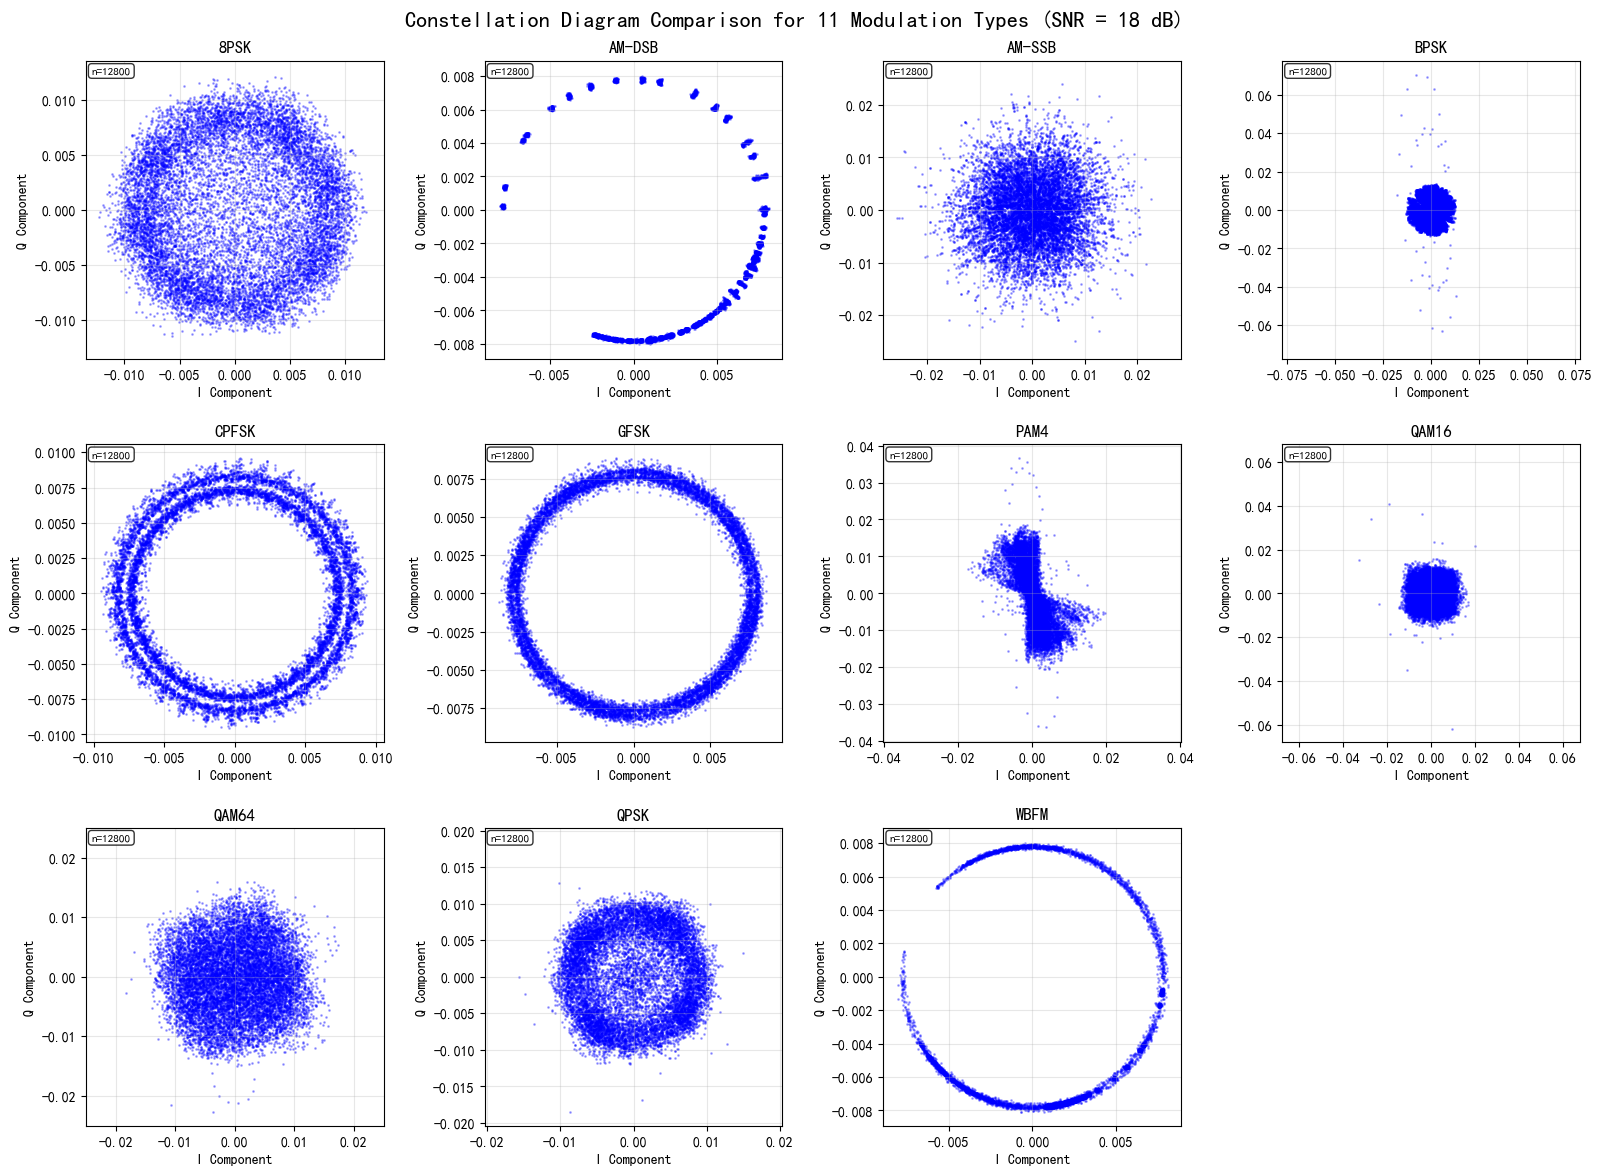
\includegraphics[width=0.45\textwidth]{figure/constellation.png}
\caption{Constellation diagrams for 11 modulation types. This figure shows the signal point distribution of each modulation scheme in the I/Q plane, the rotational symmetry of which is the basis for the rotational data augmentation strategy adopted in this study.}
\label{fig:constellation}
\end{figure}

Considering the complex attributes of digital modulated signals and the rotational symmetry of the constellation diagrams in Fig.~\ref{fig:constellation}, this study employs a rotation-based data augmentation strategy in the complex plane to enhance the model's generalization ability and robustness to phase offsets~\cite{guo2024ulcnn}.

For a complex signal \(s[n] = s_I[n] + j s_Q[n]\), rotation is achieved through the following mathematical operation. Representing the complex signal as a vector \([s_I[n], s_Q[n]]^T\), rotation is performed by multiplying with the rotation matrix \(R(\theta)\):

\begin{equation}
\begin{bmatrix} s'_I[n] \\ s'_Q[n] \end{bmatrix} = \begin{bmatrix} \cos\theta & -\sin\theta \\ \sin\theta & \cos\theta \end{bmatrix} \begin{bmatrix} s_I[n] \\ s_Q[n] \end{bmatrix}
\end{equation}

where \(s'_I[n]\) and \(s'_Q[n]\) are the rotated in-phase and quadrature components, and \(\theta\) is the rotation angle.


\begin{figure*}[htbp]
\centering
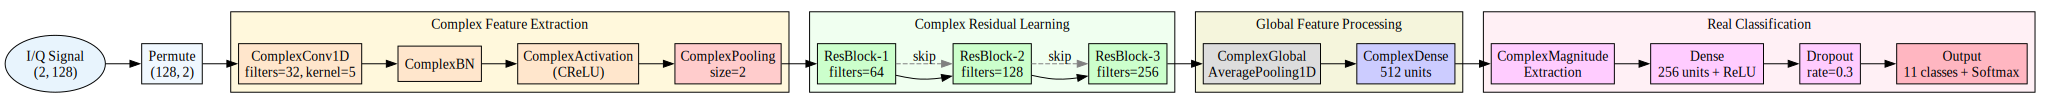
\includegraphics[width=0.85\textwidth]{figure/lightweight_hybrid_model.pdf}
\caption{Processing flow of the hybrid ComplexCNN-ResNet architecture. This figure presents a block diagram illustrating the complete processing flow from I/Q signal input, complex feature extraction, residual learning, to final modulation classification, clearly depicting the data flow and processing logic between modules.}
\label{fig:lightweight_hybrid_model_flow}
\end{figure*}


In implementation, the data augmentation algorithm takes the input data tensor \(X_{data}\) (shape \((N, 2, L)\), where \(N\) is the number of samples and \(L\) is the sequence length) and the rotation angle \(\theta_{\text{rad}}\) as parameters. It first separates the original I and Q components, applies the rotation transformation matrix, and then recombines them into augmented data samples.

Based on the symmetry of modulation types, rotations of 90° (\(\pi/2\)), 180° (\(\pi\)), and 270° (\(3\pi/2\)) are primarily used, and this strategy is applied only to modulation types with rotational symmetry (e.g., PSK, QAM). This method effectively expands the training dataset fourfold while preserving modulation features. By learning rotation-invariant feature representations, the model can better handle signal rotations caused by carrier phase offset, Doppler effect, etc.


% \begin{figure*}[htbp]
% \centering
% 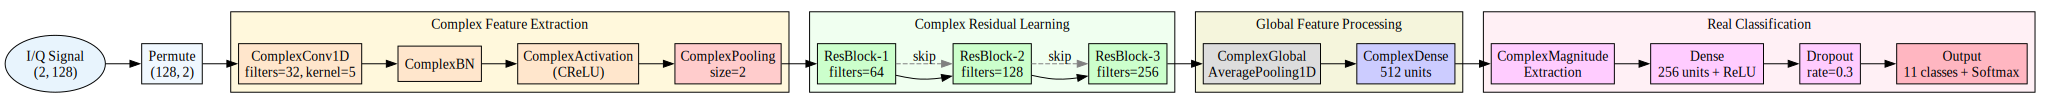
\includegraphics[width=0.85\textwidth]{figure/lightweight_hybrid_model.pdf}
% \caption{Processing flow of the hybrid ComplexCNN-ResNet architecture. This figure presents a block diagram illustrating the complete processing flow from I/Q signal input, complex feature extraction, residual learning, to final modulation classification, clearly depicting the data flow and processing logic between modules.}
% \label{fig:lightweight_hybrid_model_flow}
% \end{figure*}

\subsection{Hybrid ComplexCNN-ResNet Architecture}

\begin{figure*}[htbp]
\centering
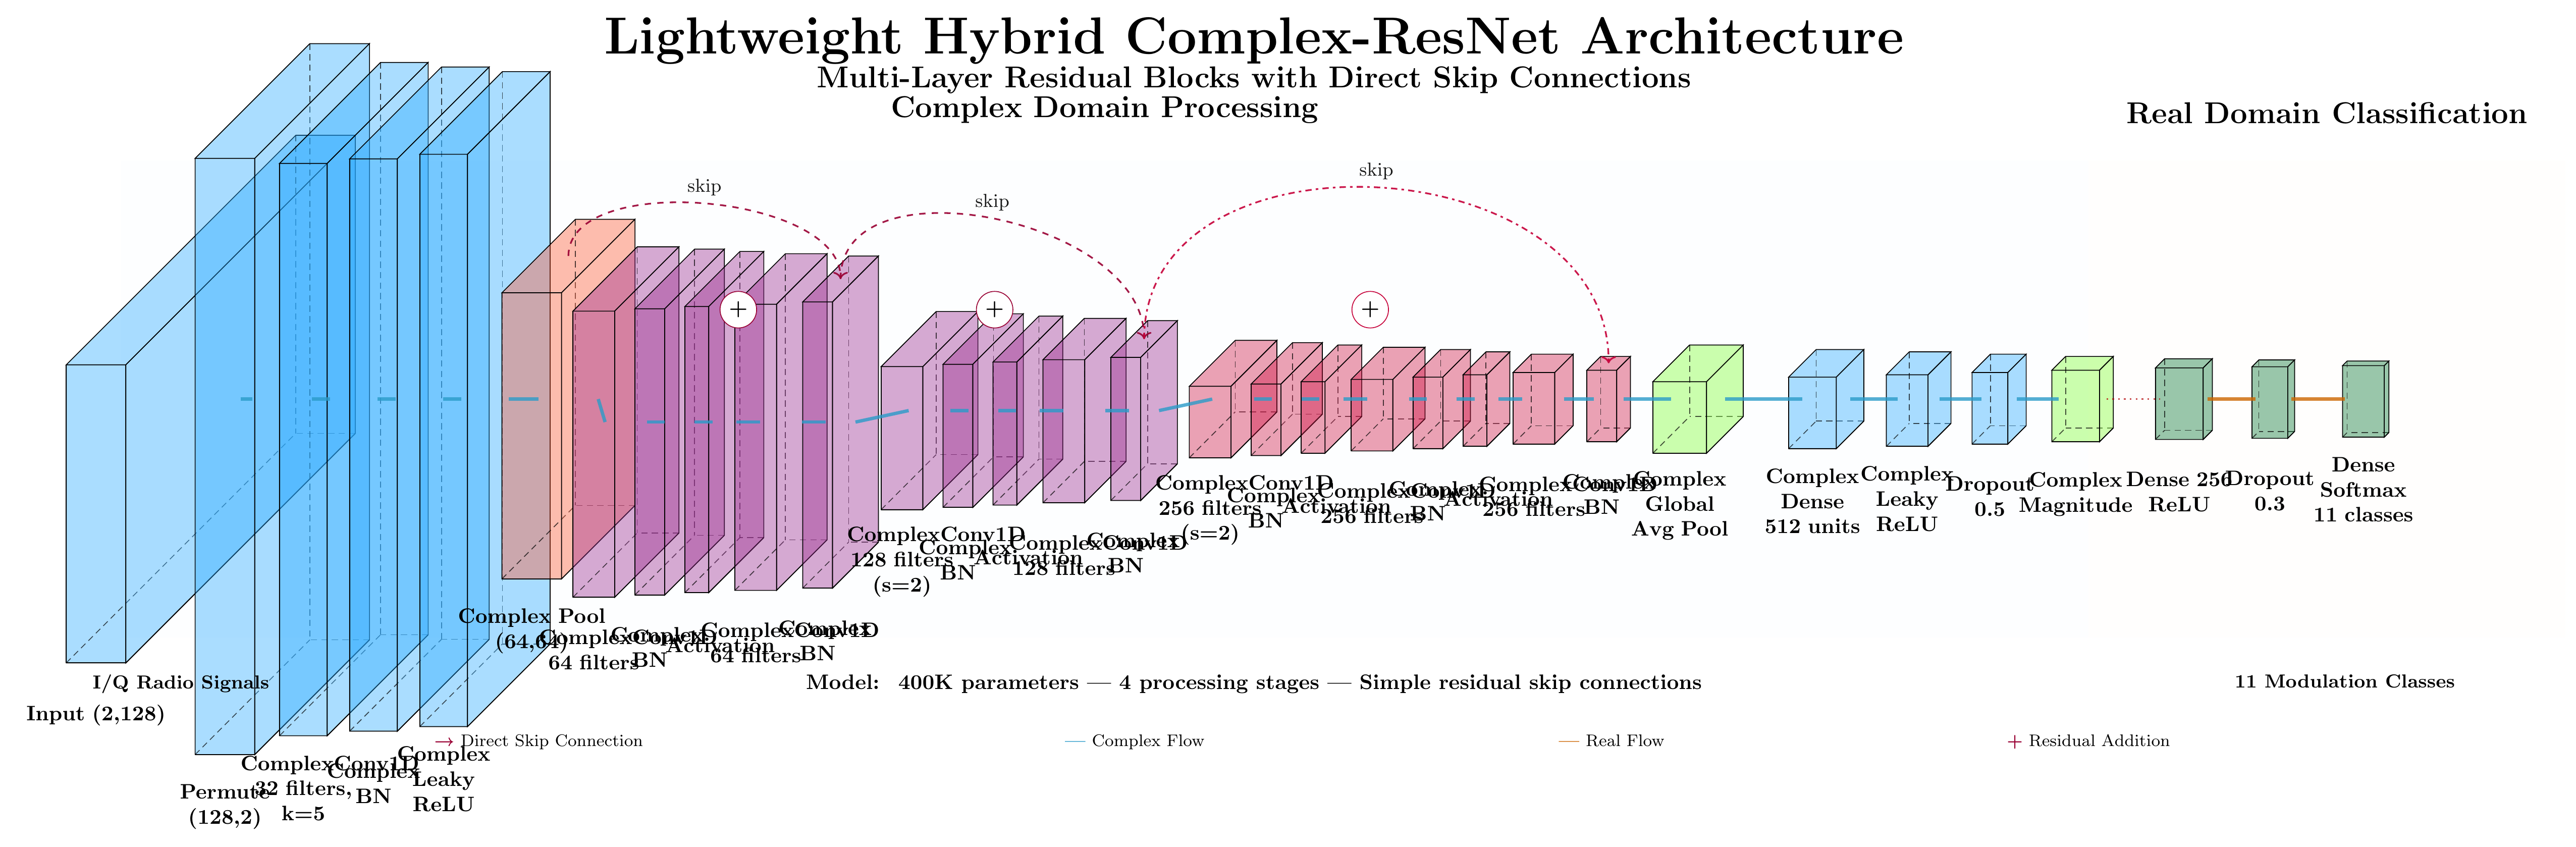
\includegraphics[width=0.9\textwidth]{figure/enhanced_hybrid_model.pdf}
\caption{Detailed architecture of the hybrid ComplexCNN-ResNet. This figure shows the complete data flow from complex input to final classification output, including complex convolutional layers, ModReLU activation function, complex residual blocks, attention mechanism, and the complex-to-real conversion process.}
\label{fig:enhanced_hybrid_model}
\end{figure*}




This paper proposes a novel hybrid ComplexCNN-ResNet architecture that fuses the fast convergence characteristics of complex neural networks with the deep feature learning capabilities of residual networks, specifically optimized for radio signal modulation classification tasks. Unlike traditional methods, this architecture maintains complex-domain operations throughout the feature extraction process, only converting to the real domain at the final classification layer, thereby maximizing the utilization of the inherent complex characteristics of I/Q signals.



\textbf{Architectural Design Principles}

The core of the hybrid architecture lies in organically unifying the initial fast convergence capability of ComplexNN with the deep feature learning capability of ResNet. ComplexNN's natural advantage in processing complex I/Q data directly preserves the integrity of the signal's amplitude and phase information, while ResNet's residual connection mechanism effectively solves the vanishing gradient problem in deep networks, enabling the model to learn more abstract discriminative features.

The architecture adopts a progressive feature extraction strategy, organizing network layers according to the principle of increasing depth of complex-domain processing:

\textbf{Complex Convolutional Layer Design} The complex convolutional layer performs true complex-domain convolution operations. For a complex input $\mathbf{a} + j\mathbf{b}$ and complex weights $\mathbf{c} + j\mathbf{d}$, the complex convolution is defined as:

\begin{align}
&(\mathbf{a} + j\mathbf{b}) * (\mathbf{c} + j\mathbf{d}) \notag \\
= &(\mathbf{a} * \mathbf{c} - \mathbf{b} * \mathbf{d}) 
+ j(\mathbf{a} * \mathbf{d} + \mathbf{b} * \mathbf{c})
\end{align}

\textbf{ModReLU Activation Function} This paper adopts the ModReLU activation function to preserve the phase information of complex signals. For a complex input $z = x + jy$, ModReLU is defined as:

\begin{equation}
|z| = \sqrt{x^2 + y^2}
\end{equation}
\begin{equation}
\phi = \arg(z) = \arctan(y/x)
\end{equation}
\begin{equation}
\text{ModReLU}(z) = \text{ReLU}(|z| + b) \cdot e^{j\phi}
\end{equation}

where $b$ is a learnable bias parameter. This activation function applies ReLU to the magnitude while completely preserving the phase information, ensuring that the geometric structure of complex features is not destroyed.

\textbf{Complex Residual Block} The complex residual block is the core innovation of the architecture, its mathematical expression is:
\begin{equation}
\mathbf{H}(z) = \mathbf{F}(z) + z
\end{equation}
where $z$ is the complex input, and $\mathbf{F}(z)$ is the learned complex residual function.

The basic residual block uses a two-layer structure:

\begin{equation}
h_1 = \text{ModReLU}(\text{CBN}(\text{CConv}(z)))
\end{equation}
\begin{equation}
h_2 = \text{CBN}(\text{CConv}(h_1))
\end{equation}
\begin{equation}
\mathbf{H}(z) = \text{ModReLU}(h_2 + z)
\end{equation}

where CBN represents Complex Batch Normalization, and CConv represents Complex Convolution.

\textbf{Complex Batch Normalization} Complex Batch Normalization standardizes the complex distribution through a whitening transformation. For a complex input $z = x + jy$, the covariance matrix is:
\begin{equation}
\mathbf{C} = \begin{bmatrix} V_{xx} & V_{xy} \\ V_{xy} & V_{yy} \end{bmatrix}
\end{equation}

The whitening matrix $\mathbf{W}$ is obtained as follows:
\begin{align}
s &= \sqrt{V_{xx}V_{yy} - V_{xy}^2} \\
t &= \sqrt{V_{xx} + V_{yy} + 2s} \\
\mathbf{W} &= \frac{1}{st}\begin{bmatrix} V_{yy} + s & -V_{xy} \\ -V_{xy} & V_{xx} + s \end{bmatrix}
\end{align}

\textbf{Advanced Residual Block with Attention Mechanism} The advanced complex residual block uses a three-layer convolutional structure and integrates complex attention:
\begin{align}
h_1 &= \text{ModReLU}(\text{CBN}(\text{CConv}(z))) \\
h_2 &= \text{ModReLU}(\text{CBN}(\text{CConv}(h_1))) \\
h_3 &= \text{CBN}(\text{CConv}_{1 \times 1}(h_2))
\end{align}

The complex attention weights are calculated as:
\begin{equation}
\mathbf{A} = \text{Tanh}(\text{CConv}_{1 \times 1}(h_3))
\end{equation}

The final output is:
\begin{equation}
\mathbf{H}(z) = \text{ModReLU}(h_3 \odot \mathbf{A} + z_{shortcut})
\end{equation}
where $\odot$ represents complex element-wise multiplication.

\textbf{Global Feature Aggregation} Complex global average pooling aggregates temporal features into a global representation:
\begin{equation}
f_{global} = \frac{1}{T} \sum_{t=1}^T z_t
\end{equation}

\textbf{Complex to Real Conversion} Finally, conversion to the real domain is done by extracting the magnitude:
\begin{equation}
|z| = \sqrt{x^2 + y^2 + \epsilon}
\end{equation}
where $\epsilon$ is a numerical stability term.

The main advantages of this hybrid architecture include: (1) complete preservation of the complex characteristics and phase information of I/Q signals; (2) residual connections ensure effective training of deep networks; (3) the ModReLU activation function maintains phase integrity during non-linear transformations; (4) lightweight design significantly reduces computational complexity while maintaining performance. Through this carefully designed hybrid architecture, the model can fully exploit the intrinsic structural features of I/Q signals, achieving accurate classification of different modulation types.

\section{Experimental Setup}

\subsection{Training Configuration}

All experiments in this study were conducted on a high-performance workstation equipped with an Intel Core i9-13900K processor, an NVIDIA GeForce RTX 4090 GPU (24GB GDDR6X memory), and 64GB of system memory. The deep learning framework used was TensorFlow 2.17.0 and Keras 3.6.0, with CUDA 12.4 and cuDNN 9.1.1.17 for GPU-accelerated computation. The operating system was Ubuntu 24.04.2 LTS.

\textbf{Hyperparameter Settings:}
All models were trained with a unified configuration to ensure fair comparison. The learning rate was set to 0.001, using the Adam optimizer, with a batch size of 128. The training process employed an early stopping mechanism, stopping training if the validation set accuracy did not improve for 30 consecutive epochs, with a maximum of 200 training epochs. To prevent overfitting, Dropout regularization was used in the fully connected layers with a dropout rate of 0.5.

\textbf{Learning Rate Scheduling:}
A stepped learning rate decay strategy was adopted. The initial learning rate was 0.001, and if the validation set accuracy did not improve within 5 epochs, it was decayed to 0.5 times its current value, with a minimum learning rate set to 1e-6. This scheduling strategy helps the model to fine-tune in the later stages of training.

\textbf{Data Splitting Strategy:}
The dataset was divided into training, validation, and test sets at a ratio of 72\%:8\%:20\%, ensuring a uniform distribution of each modulation type and SNR condition across the three sets. The validation set was used for hyperparameter tuning and model selection, while the test set was used only for final performance evaluation.

\textbf{Training Procedure:}
For evaluating the improved methods, a progressive training strategy was adopted: first, the baseline model was trained, then GPR denoising, rotational data augmentation, and the hybrid architecture were added sequentially. Each stage was trained independently, and performance improvements were recorded. Finally, the complete model incorporating all improvements was trained.

\subsection{Evaluation Metrics}

This study employs a multi-dimensional evaluation system to comprehensively analyze the performance of the proposed method.

\textbf{Classification Accuracy:}
The primary evaluation metric is overall classification accuracy, defined as the ratio of correctly classified samples to the total number of samples:
\begin{equation}
\text{Accuracy} = \frac{N_{correct}}{N_{total}} \times 100\%
\end{equation}

\textbf{Performance Analysis under SNR Conditions:}
To evaluate the model's robustness under different noise conditions, the test set was divided into three subsets based on SNR range: low SNR (-20dB to -2dB), medium SNR (0dB to 8dB), and high SNR (10dB to 18dB). Accuracy was calculated separately for each subset.

\textbf{Confusion Matrix Analysis:}
The classification performance for each modulation type was analyzed using a confusion matrix, calculating the Precision, Recall, and F1-score for each class:

\begin{equation}
\text{Precision} = \frac{TP}{TP + FP}
\end{equation}
\begin{equation}
\text{Recall} = \frac{TP}{TP + FN}
\end{equation}
\begin{equation}
\text{F1-Score} = \frac{2 \times \text{Precision} \times \text{Recall}}{\text{Precision} + \text{Recall}}
\end{equation}

where TP, FP, and FN represent the number of true positives, false positives, and false negatives, respectively.

\section{Results and Analysis}

\subsection{Baseline Performance Comparison}

To validate the effectiveness of the proposed hybrid architecture, we first evaluated the performance of several baseline models on the RML2016.10a dataset, including Fully Connected Neural Network (FCNN), 1D Convolutional Neural Network (CNN1D), 2D Convolutional Neural Network (CNN2D), Residual Network (ResNet), Transformer, and Complex Convolutional Neural Network (ComplexCNN).

Table~\ref{tab:baseline_comparison} shows the performance comparison of various baseline models under the same training conditions. The experimental results indicate significant differences in classification performance among different architectures. The ResNet architecture, due to its residual connection mechanism effectively alleviating the vanishing gradient problem, demonstrated excellent convergence characteristics in deep network training, achieving a classification accuracy of 55.37\%. ComplexCNN has a natural advantage in processing complex I/Q signals, better preserving the phase information of the signal, and obtained an accuracy of 57.11\%.

\begin{table}[!htbp]
\centering
\caption{Baseline Model Performance Comparison}
\label{tab:baseline_comparison}
\begin{tabular}{@{}cc@{}}
\toprule
Model Architecture & Accuracy (\%) \\
\midrule
FCNN & 42.65 \\
CNN2D & 47.31 \\
Transformer & 47.86 \\
CNN1D & 54.94 \\
ResNet & 55.37 \\
ComplexCNN & 57.11 \\
\bottomrule
\end{tabular}
\end{table}

\begin{figure}[htbp]
\centering
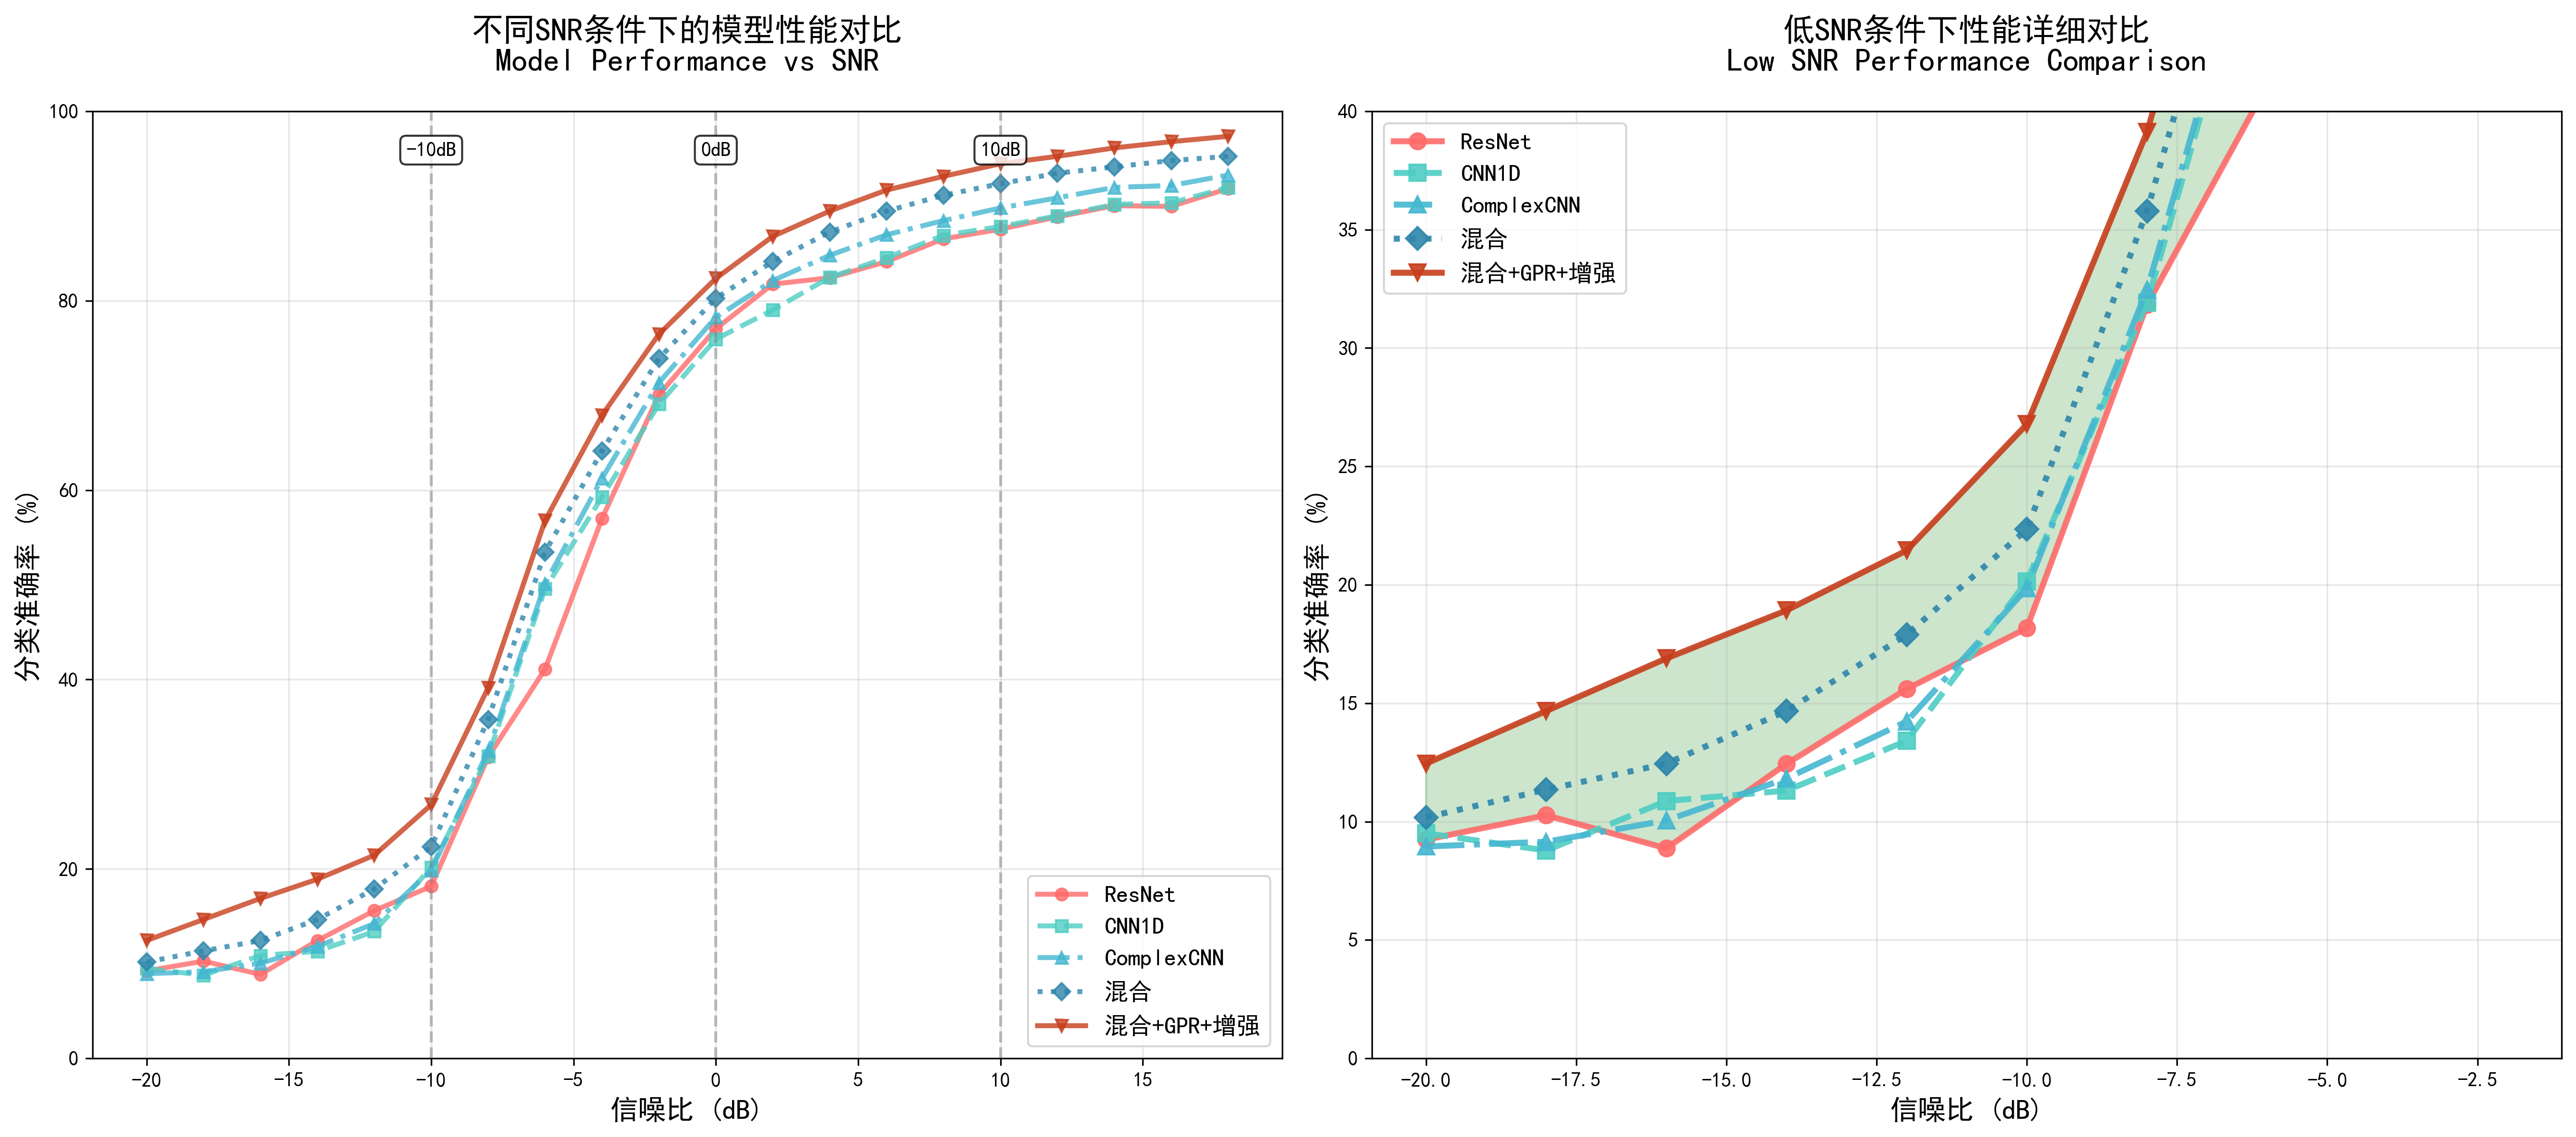
\includegraphics[width=0.45\textwidth]{figure/snr_performance_comparison.pdf}
\caption{Performance comparison of different models under various SNR conditions. The figure shows the classification accuracy curves of five models (CNN1D, ResNet, ComplexCNN, Hybrid Architecture, Hybrid Architecture+GPR+Augmentation) under different signal-to-noise ratio conditions.}
\label{fig:snr_performance}
\end{figure}

Fig.~\ref{fig:snr_performance} shows the performance curves of different baseline models under various SNR conditions. It can be observed that all models experience a significant performance drop under low SNR conditions, but ComplexCNN and ResNet perform relatively stably under medium to high SNR conditions, which provided an important reference for our hybrid architecture design.

Based on the results and analysis of these baseline experiments, we designed a hybrid architecture that integrates the residual learning capability of ResNet with the complex processing advantages of ComplexCNN. This hybrid model, combined with GPR denoising and rotational data augmentation techniques, ultimately achieved a classification accuracy of 65.38\% on the RML2016.10a dataset, a significant improvement of 8.27 percentage points compared to the best single baseline architecture (ComplexCNN).

\begin{figure}[htbp]
\centering
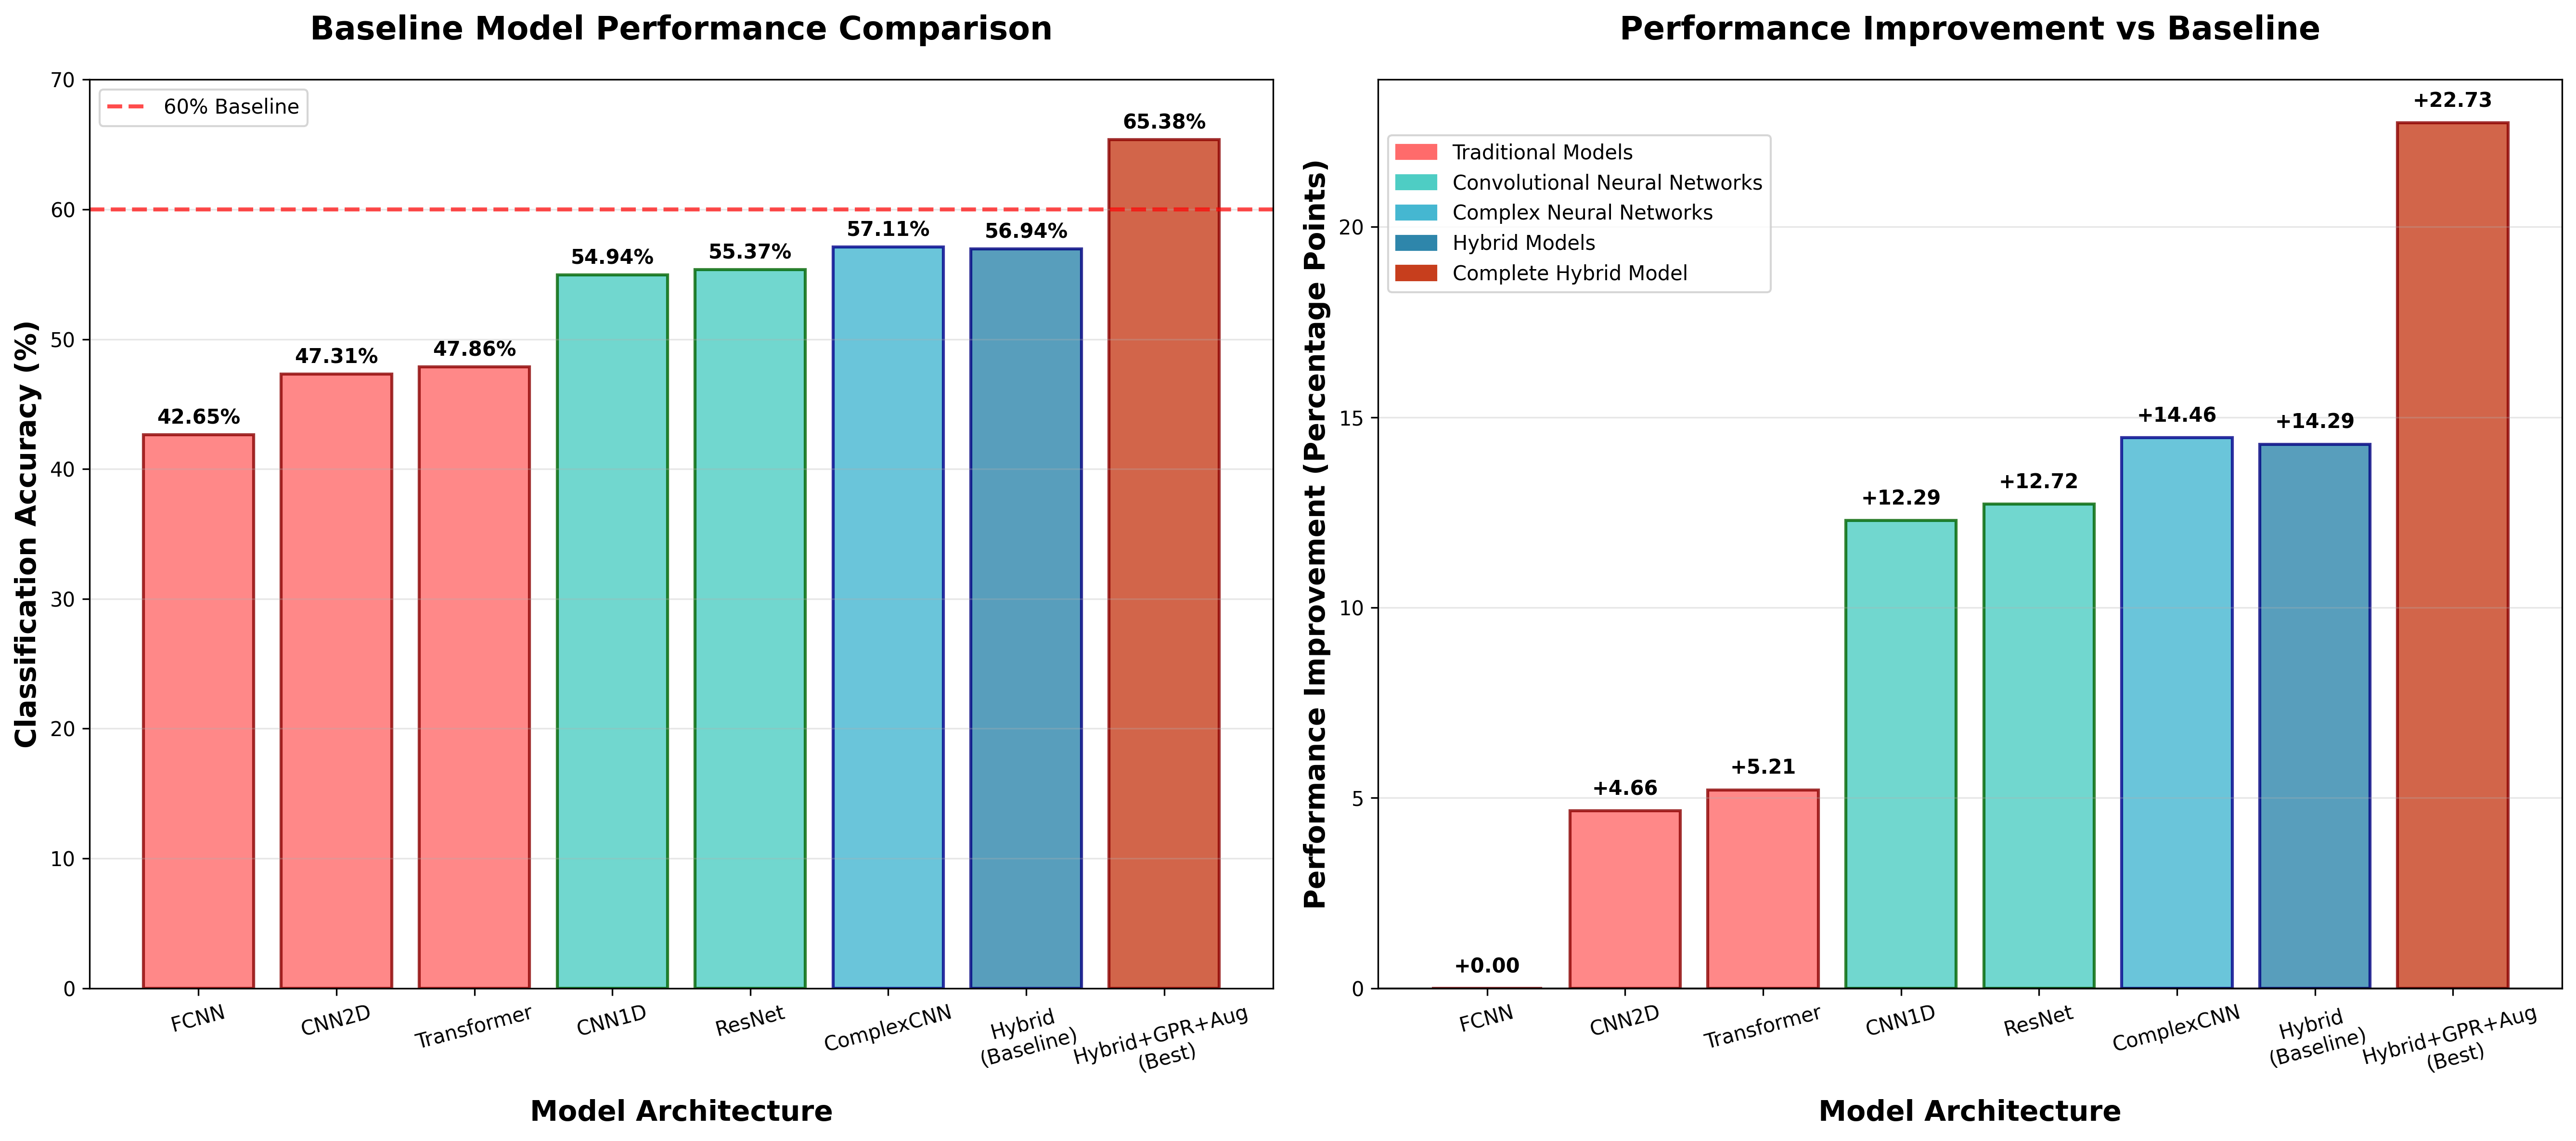
\includegraphics[width=0.45\textwidth]{figure/baseline_model_comparison.pdf}
\caption{Performance comparison analysis of different model architectures. This figure presents a comprehensive comparison of the hybrid architecture with traditional baseline models on key metrics such as classification accuracy, number of model parameters, and inference time.}
\label{fig:model_comparison}
\end{figure}

\subsection{Impact of Gaussian Process Regression Denoising}
GPR denoising technology played a significant role in improving model performance, demonstrating notable improvements across all SNR conditions. Fig.~\ref{fig:constellation_denoising} shows a comparison of signal quality before and after GPR denoising, clearly illustrating the effective suppression of noise.

Table~\ref{tab:gpr_impact} provides a detailed analysis of the impact of GPR denoising on classification accuracy across different SNR ranges. The experimental results show that GPR denoising led to a 7.25 percentage point performance increase in low SNR conditions (-20dB to -8dB), a 5.12 percentage point increase in medium SNR conditions (-6dB to 4dB), and a 5.07 percentage point increase in high SNR conditions (6dB to 18dB). Overall, GPR denoising improved the accuracy of the hybrid architecture from 56.94\% to 62.80\%, achieving a significant improvement of 5.86 percentage points. This result indicates that GPR denoising technology provides stable and considerable performance gains across all SNR ranges, with the largest absolute improvement observed in low SNR conditions, highlighting the importance of denoising techniques in adverse channel environments.

\begin{table}[!htbp]
\centering
\caption{Impact of GPR Denoising on Different SNR Ranges}
\label{tab:gpr_impact}
\begin{threeparttable}
\begin{tabular}{@{}cccc@{}}
\toprule
SNR Range & Before (\%) & After (\%) & Improvement (\%) \\
\midrule
Low SNR$^{a}$ & 15.14 & 22.40 & +7.25 \\
Mid SNR$^{b}$ & 73.58 & 78.70 & +5.12 \\
High SNR$^{c}$ & 84.15 & 89.23 & +5.07 \\
Overall & 56.94 & 62.80 & +5.86 \\
\bottomrule
\end{tabular}
\begin{tablenotes}
\footnotesize
\item[$^{a}$] Low SNR: -20dB to -8dB
\item[$^{b}$] Mid SNR: -6dB to 4dB  
\item[$^{c}$] High SNR: 6dB to 18dB
\end{tablenotes}
\end{threeparttable}
\end{table}

\begin{figure}[htbp]
\centering
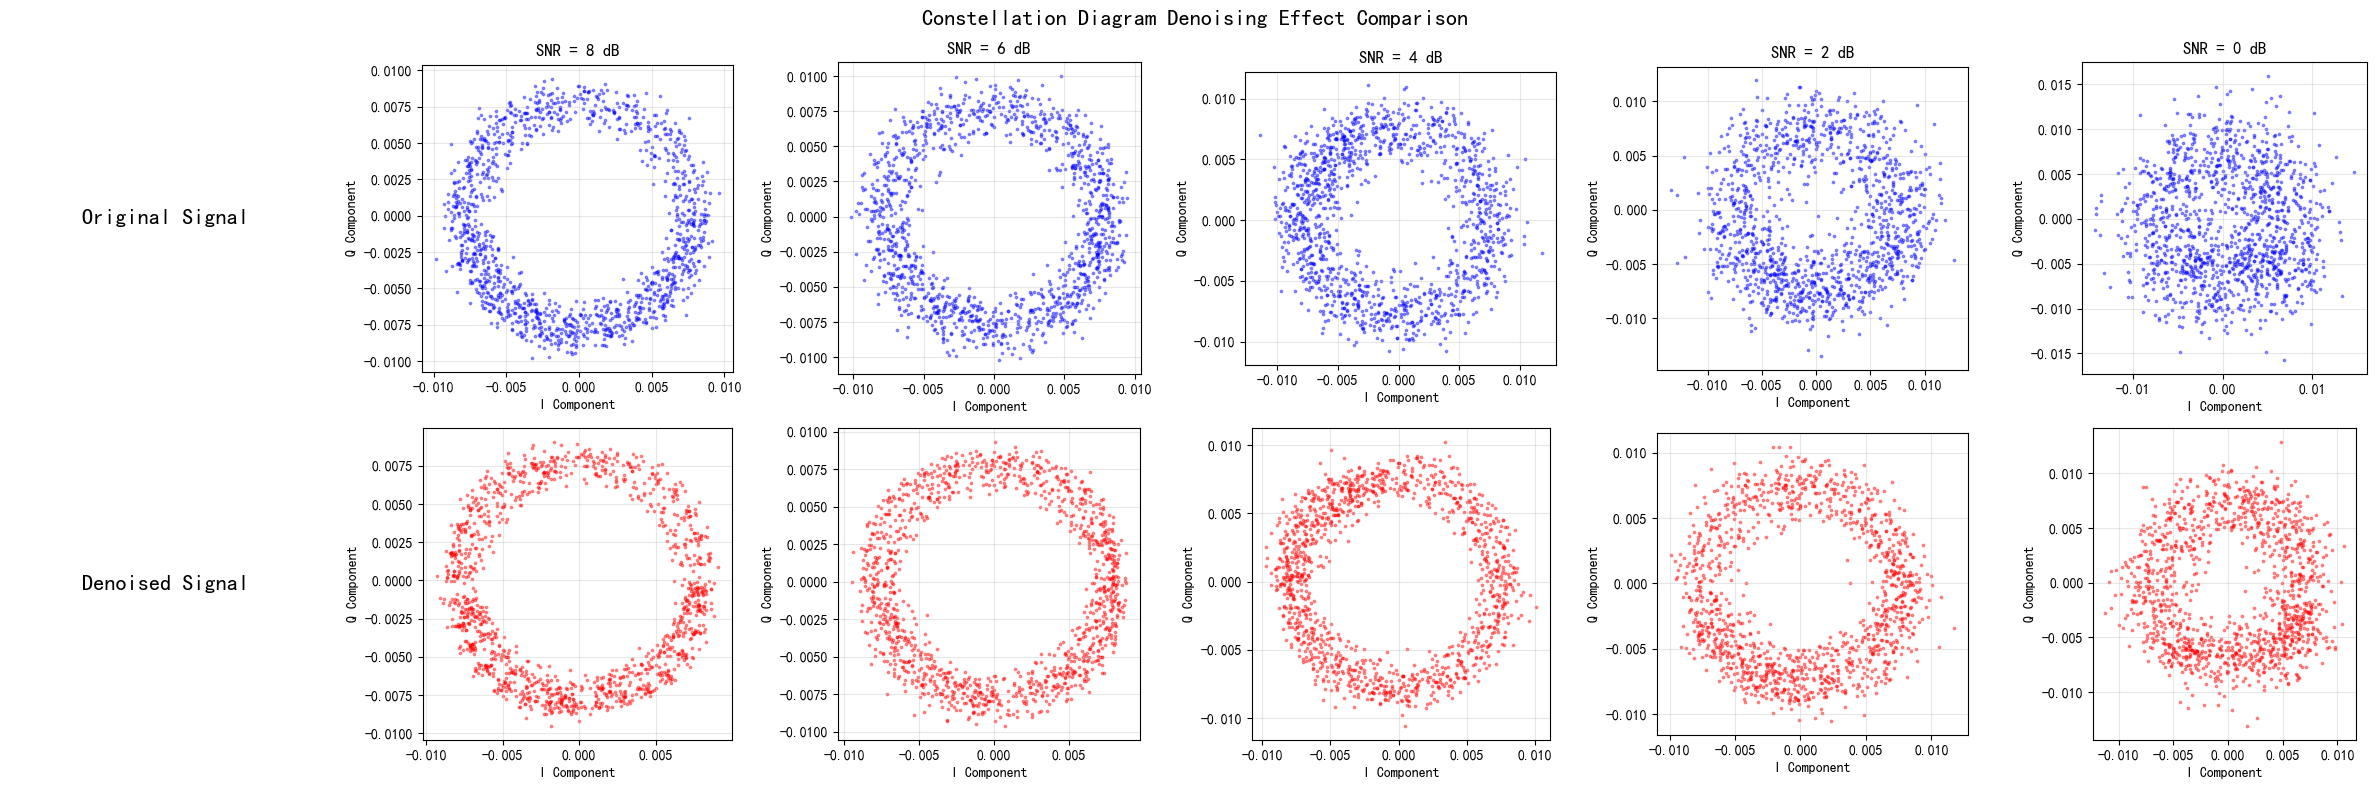
\includegraphics[width=0.45\textwidth]{figure/constellation_denoising.png}
\caption{Denoising effect on the constellation diagram of CPFSK modulation type under SNR conditions of 0 to 8dB.}
\label{fig:constellation_denoising}
\end{figure}

Fig.~\ref{fig:constellation_denoising} shows the denoising effect on the constellation diagram of the CPFSK modulation type under SNR conditions of 0 to 8dB. It can be seen from the figure that GPR denoising effectively preserves the structural features of the signal while significantly reducing the noise impact, which lays a good foundation for subsequent deep learning classification.

Table~\ref{tab:gpr_detailed_snr} provides a more detailed analysis of the GPR denoising effect, showing the change in classification accuracy at each specific SNR value. It is clear from the table that GPR denoising brings greater improvements under low SNR conditions. As SNR increases, the improvement margin shows a complex pattern of change. In extremely low SNR conditions (-20dB to -18dB), the improvement is relatively small (1.03\% to 1.54\%); whereas in low to medium SNR conditions (-12dB to -10dB), the improvement effect peaks, achieving significant gains of 11.53\% and 14.90\%, respectively. Under medium SNR conditions (0dB), accuracy increased from 79.43\% to 83.17\%, an improvement of 3.74\%; under high SNR conditions (18dB), accuracy increased from 83.87\% to 88.98\%, an improvement of 5.11\%. This trend indicates that GPR denoising is most effective in low to medium SNR conditions, with relatively moderate improvements in extremely low and high SNR conditions, consistent with theoretical expectations in signal processing.



% \begin{table}[!htbp]
% \centering
% \caption{Detailed Impact of GPR Denoising at Various SNR Levels}
% \label{tab:gpr_detailed_snr}
% \begin{tabular}{@{}cccc@{}}
% \toprule
% SNR (dB) & Baseline (\%) & Baseline+GPR (\%) & Improvement (\%) \\
% \midrule
% -20 & 8.93 & 9.96 & +1.03 \\
% -18 & 8.68 & 10.22 & +1.54 \\
% -16 & 9.85 & 12.69 & +2.84 \\
% -14 & 11.08 & 17.32 & +6.24 \\
% -12 & 12.65 & 24.18 & +11.53 \\
% -10 & 20.15 & 35.05 & +14.90 \\
% -8 & 34.66 & 47.36 & +12.70 \\
% -6 & 54.86 & 61.21 & +6.35 \\
% -4 & 64.02 & 70.84 & +6.82 \\
% -2 & 75.66 & 80.89 & +5.23 \\
% 0 & 79.43 & 83.17 & +3.74 \\
% 2 & 82.96 & 87.07 & +4.11 \\
% 4 & 84.56 & 89.00 & +4.44 \\
% 6 & 83.93 & 89.38 & +5.45 \\
% 8 & 83.17 & 89.10 & +5.93 \\
% 10 & 84.73 & 89.85 & +5.12 \\
% 12 & 85.81 & 90.31 & +4.50 \\
% 14 & 85.31 & 88.81 & +3.50 \\
% 16 & 82.25 & 88.15 & +5.90 \\
% 18 & 83.87 & 88.98 & +5.11 \\
% \bottomrule
% \end{tabular}
% \end{table}

% \textbf{Note:} In the table, "Baseline" refers to the hybrid architecture, and "Baseline+GPR" refers to the hybrid architecture with GPR denoising added.

\begin{table}[!htbp]
\centering
\caption{Detailed Impact of GPR Denoising at Various SNR Levels}
\label{tab:gpr_detailed_snr}
\begin{threeparttable}
\begin{tabular}{@{}cccc@{}}
\toprule
SNR (dB) & Baseline (\%) & Baseline+GPR (\%) & Improvement (\%) \\
\midrule
-20 & 8.93 & 9.96 & +1.03 \\
-18 & 8.68 & 10.22 & +1.54 \\
-16 & 9.85 & 12.69 & +2.84 \\
-14 & 11.08 & 17.32 & +6.24 \\
-12 & 12.65 & 24.18 & +11.53 \\
-10 & 20.15 & 35.05 & +14.90 \\
-8 & 34.66 & 47.36 & +12.70 \\
-6 & 54.86 & 61.21 & +6.35 \\
-4 & 64.02 & 70.84 & +6.82 \\
-2 & 75.66 & 80.89 & +5.23 \\
0 & 79.43 & 83.17 & +3.74 \\
2 & 82.96 & 87.07 & +4.11 \\
4 & 84.56 & 89.00 & +4.44 \\
6 & 83.93 & 89.38 & +5.45 \\
8 & 83.17 & 89.10 & +5.93 \\
10 & 84.73 & 89.85 & +5.12 \\
12 & 85.81 & 90.31 & +4.50 \\
14 & 85.31 & 88.81 & +3.50 \\
16 & 82.25 & 88.15 & +5.90 \\
18 & 83.87 & 88.98 & +5.11 \\
\bottomrule
\end{tabular}
\begin{tablenotes}
\item[] \textbf{Note:} In the table, "Baseline" refers to the hybrid architecture, and "Baseline+GPR" refers to the hybrid architecture with GPR denoising added.
\end{tablenotes}
\end{threeparttable}
\end{table}




\subsection{Effect of Rotation-based Data Augmentation}

The rotation-based data augmentation strategy in the complex plane significantly improved the model's generalization ability and robustness to phase offsets. This technique utilizes the rotational symmetry of digital modulation signal constellation diagrams, expanding the training dataset to four times its original size through 90°, 180°, and 270° rotational transformations.

Table~\ref{tab:data_augmentation_results} shows the impact of data augmentation on the classification performance of different modulation types. The experimental results indicate that rotational data augmentation yields the most significant performance improvements for QAM-type modulations (QAM16, QAM64) and some PSK-type modulations. The accuracy for QAM16 increased substantially from a baseline of 46\% to 68\%, an improvement of 22 percentage points; QAM64 improved from 54\% to 75\%, an increase of 21 percentage points. For 8PSK, accuracy rose from 72\% to 82\%, a 10 percentage point increase; BPSK improved from 72\% to 80\%, an 8 percentage point increase. GFSK also showed significant improvement, from 76\% to 88\%, an increase of 12 percentage points. Overall, rotational data augmentation increased the accuracy of the hybrid architecture from 56.94\% to 60.72\%, achieving a notable improvement of 3.78 percentage points.

\begin{table}[!htbp]
\centering
\caption{Impact of Data Augmentation on Various Modulation Types}
\label{tab:data_augmentation_results}
\begin{tabular}{@{}cccc@{}}
\toprule
Modulation & Baseline (\%) & Augmented (\%) & Improvement (\%) \\
\midrule
8PSK     & 72  & 82  & +10 \\
AM-DSB   & 54  & 57  & +3  \\
AM-SSB   & 27  & 26  & -1  \\
BPSK     & 72  & 80  & +8  \\
CPFSK    & 82  & 88  & +6  \\
GFSK     & 76  & 88  & +12 \\
PAM4     & 92  & 93  & +1  \\
QAM16    & 46  & 68  & +22 \\
QAM64    & 54  & 75  & +21 \\
QPSK     & 84  & 75  & -9  \\
WBFM     & 82  & 85  & +3  \\
\bottomrule
\end{tabular}
\end{table}

\begin{figure}[htbp]
\centering
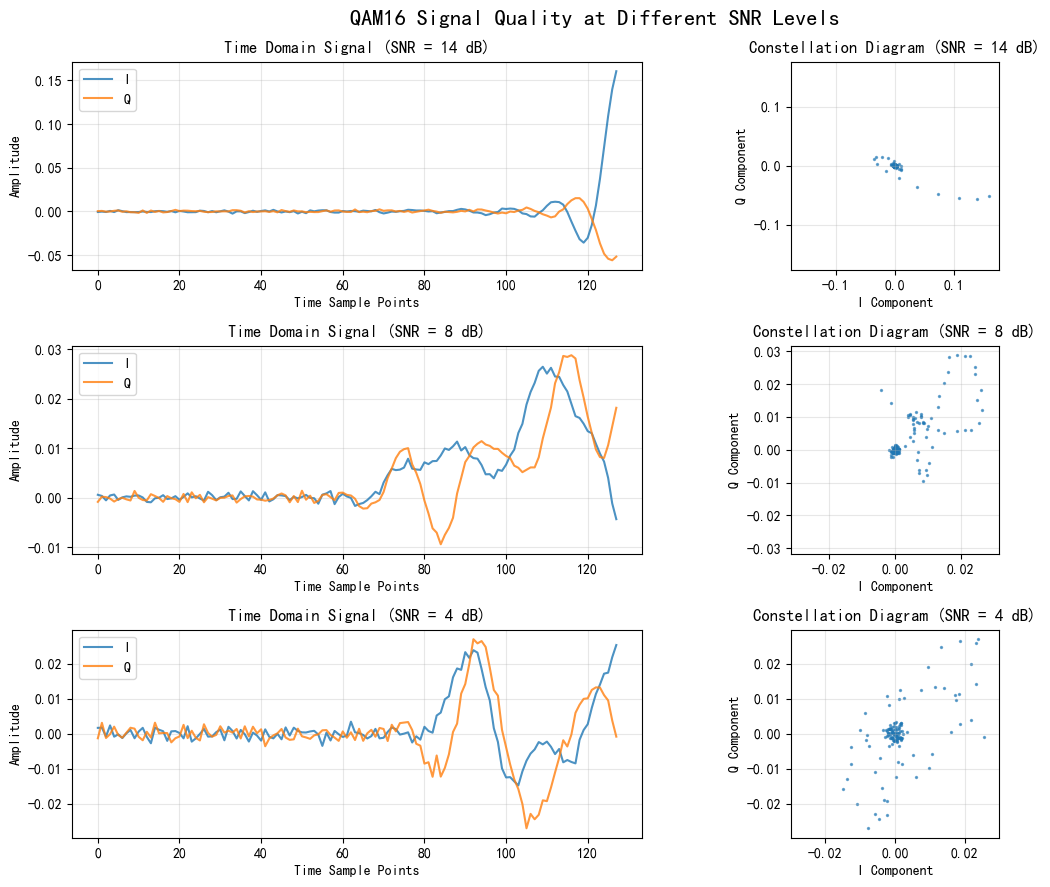
\includegraphics[width=0.45\textwidth]{figure/QAM16_rotation.png}
\caption{I/Q channel plot and constellation diagram for QAM16 signal.}
\label{fig:rotation_augmentation}
\end{figure}

Fig.~\ref{fig:rotation_augmentation} shows the I/Q channel plots and constellation diagrams for some QAM16 signals. From the constellation diagrams, it can be observed that a single signal has a clear directional nature. Rotational transformation can enhance the information of the signal in different directions, providing the model with richer training samples. This augmentation strategy is particularly effective in addressing signal rotation issues caused by factors such as carrier phase offset and local oscillator frequency deviation in practical communication environments.

% Further analysis of model robustness showed that models trained with rotational data augmentation exhibited greater stability when faced with artificial phase offsets introduced during testing. When test signals were randomly rotated from 0° to 360°, the average accuracy drop for the augmented model was only 1.8\%, whereas the baseline model without augmentation experienced an accuracy drop of up to 7.3\%. This demonstrates the effectiveness of rotational data augmentation in enhancing the model's practical application performance.

\subsection{Hybrid Architecture Performance}

The proposed hybrid ComplexCNN-ResNet architecture achieved significant performance improvement on the RML2016.10a dataset, with a final classification accuracy of 65.38\%. This is an 8.27~percentage point increase compared to the 57.11\% accuracy of the best single baseline architecture, ComplexCNN.

Fig~\ref{fig:method_comparison} and Table~\ref{tab:hybrid_performance} presents a detailed performance comparison of the hybrid architecture with existing advanced methods. A thorough analysis of the results reveals a remarkable transformation in model performance. Initially, substantial performance gaps existed between the baseline models and state-of-the-art methods. However, the systematic integration of Gaussian Process Regression (GPR) denoising and rotation-based data augmentation techniques fundamentally transformed the performance landscape. The enhanced versions of ResNet, ComplexCNN, and the hybrid ComplexCNN-ResNet architecture all achieved performance levels that either matched or surpassed existing advanced methods. 

An in-depth examination of Fig~\ref{fig:method_comparison} reveals interesting architectural dynamics that motivated our hybrid design approach. Initially, ComplexCNN demonstrated superior classification accuracy compared to ResNet in the baseline configuration. However, a notable performance reversal occurred when GPR denoising and rotation-based data augmentation were applied: ResNet began to outperform ComplexCNN under these enhanced conditions. This phenomenon suggests that ResNet's deeper residual structure possesses a greater capacity to extract meaningful patterns from GPR-denoised data, effectively leveraging the improved signal quality provided by the preprocessing techniques. Recognizing this complementary behavior, we developed the hybrid ComplexCNN-ResNet architecture to harness the strengths of both approaches. While the baseline hybrid model achieved performance slightly below that of the standalone ComplexCNN (though remaining very competitive), the integration of GPR denoising and rotation data augmentation enabled the hybrid architecture to surpass both the enhanced ComplexCNN (63.41\%) and enhanced ResNet (64.37\%), ultimately achieving our best performance of 65.38\% and exceeding the previous state-of-the-art benchmark of 64.59\%.

The experimental results demonstrate that the proposed hybrid method outperforms existing methods across multiple dimensions, including accuracy, parameter efficiency, and training stability.Most notably, the optimized hybrid ComplexCNN-ResNet architecture successfully surpassed the previous state-of-the-art performance established by AbFTNet (64.59\%), achieving a new benchmark accuracy of 65.38\% and establishing itself as the new state-of-the-art (SOTA) method in automatic modulation classification. Compared to Ultra Lite CNN (ULCNN) with 62.47\% accuracy, our method improves by 2.91~percentage points; compared to AMC-NET with 62.51\%, it improves by 2.87~percentage points; and compared to the previous SOTA AbFTNet with 64.59\%, it achieves a meaningful improvement of 0.79~percentage points.

\begin{figure}[htbp]
\centering
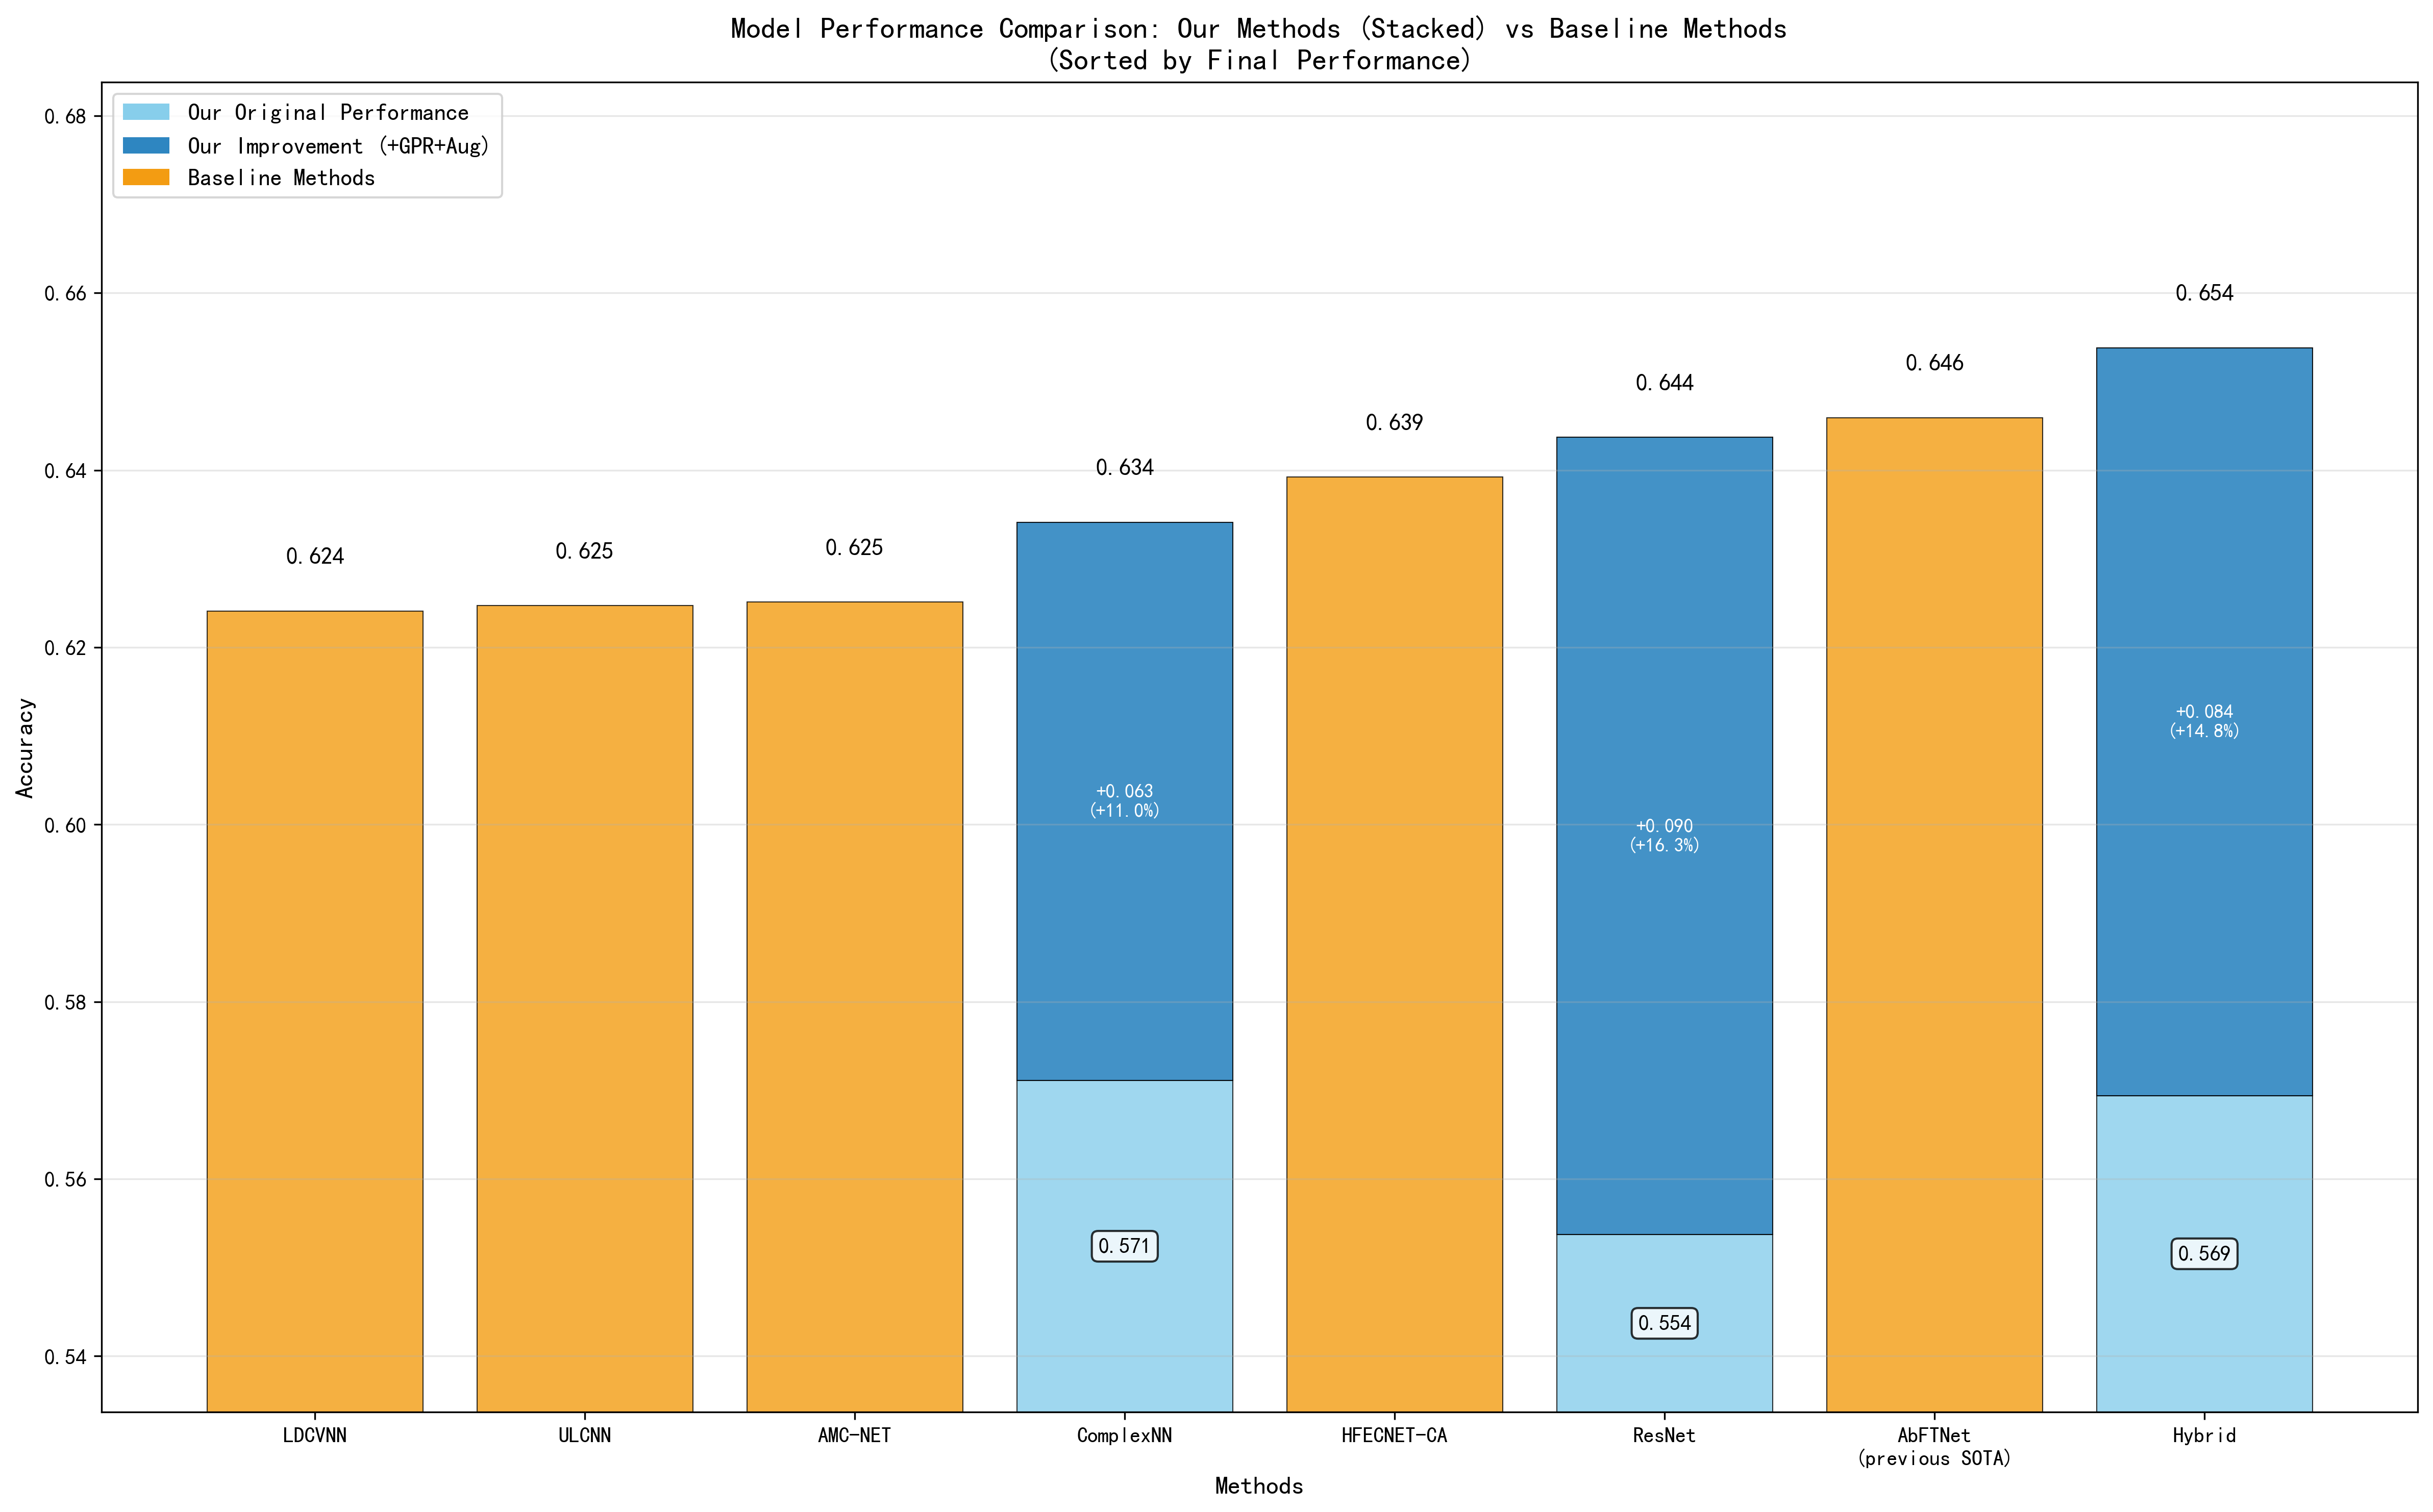
\includegraphics[width=0.45\textwidth]{figure/sorted_stacked_comparison.png}
\caption{Comprehensive performance comparison analysis of different methods. This figure displays the performance of various technical solutions sorted by classification accuracy, clearly reflecting the superiority of the comprehensive method proposed in this study.}
\label{fig:method_comparison}
\end{figure}

\begin{table}[!htbp]
\centering
\caption{Performance Comparison of Hybrid Architecture with Existing Methods}
\label{tab:hybrid_performance}
\begin{tabular}{@{}cc@{}}
\toprule
Method & Accuracy (\%) \\
\midrule
LDCVNN~\cite{xu2025ldcvnn} & 62.41 \\
ULCNN~\cite{guo2024ulcnn} & 62.47 \\
AMC-NET~\cite{zhang2023amcnet} & 62.51 \\
HFECNET-CA~\cite{ma2023hfecnetca} & 63.92 \\
AbFTNet~\cite{ning2024abftnet} \textbf{(previous SOTA)} & 64.59 \\
\textbf{GRCR-Net (Proposed Method)} & \textbf{65.38} \\
\bottomrule
\end{tabular}
\end{table}


\begin{figure}[htbp]
\centering
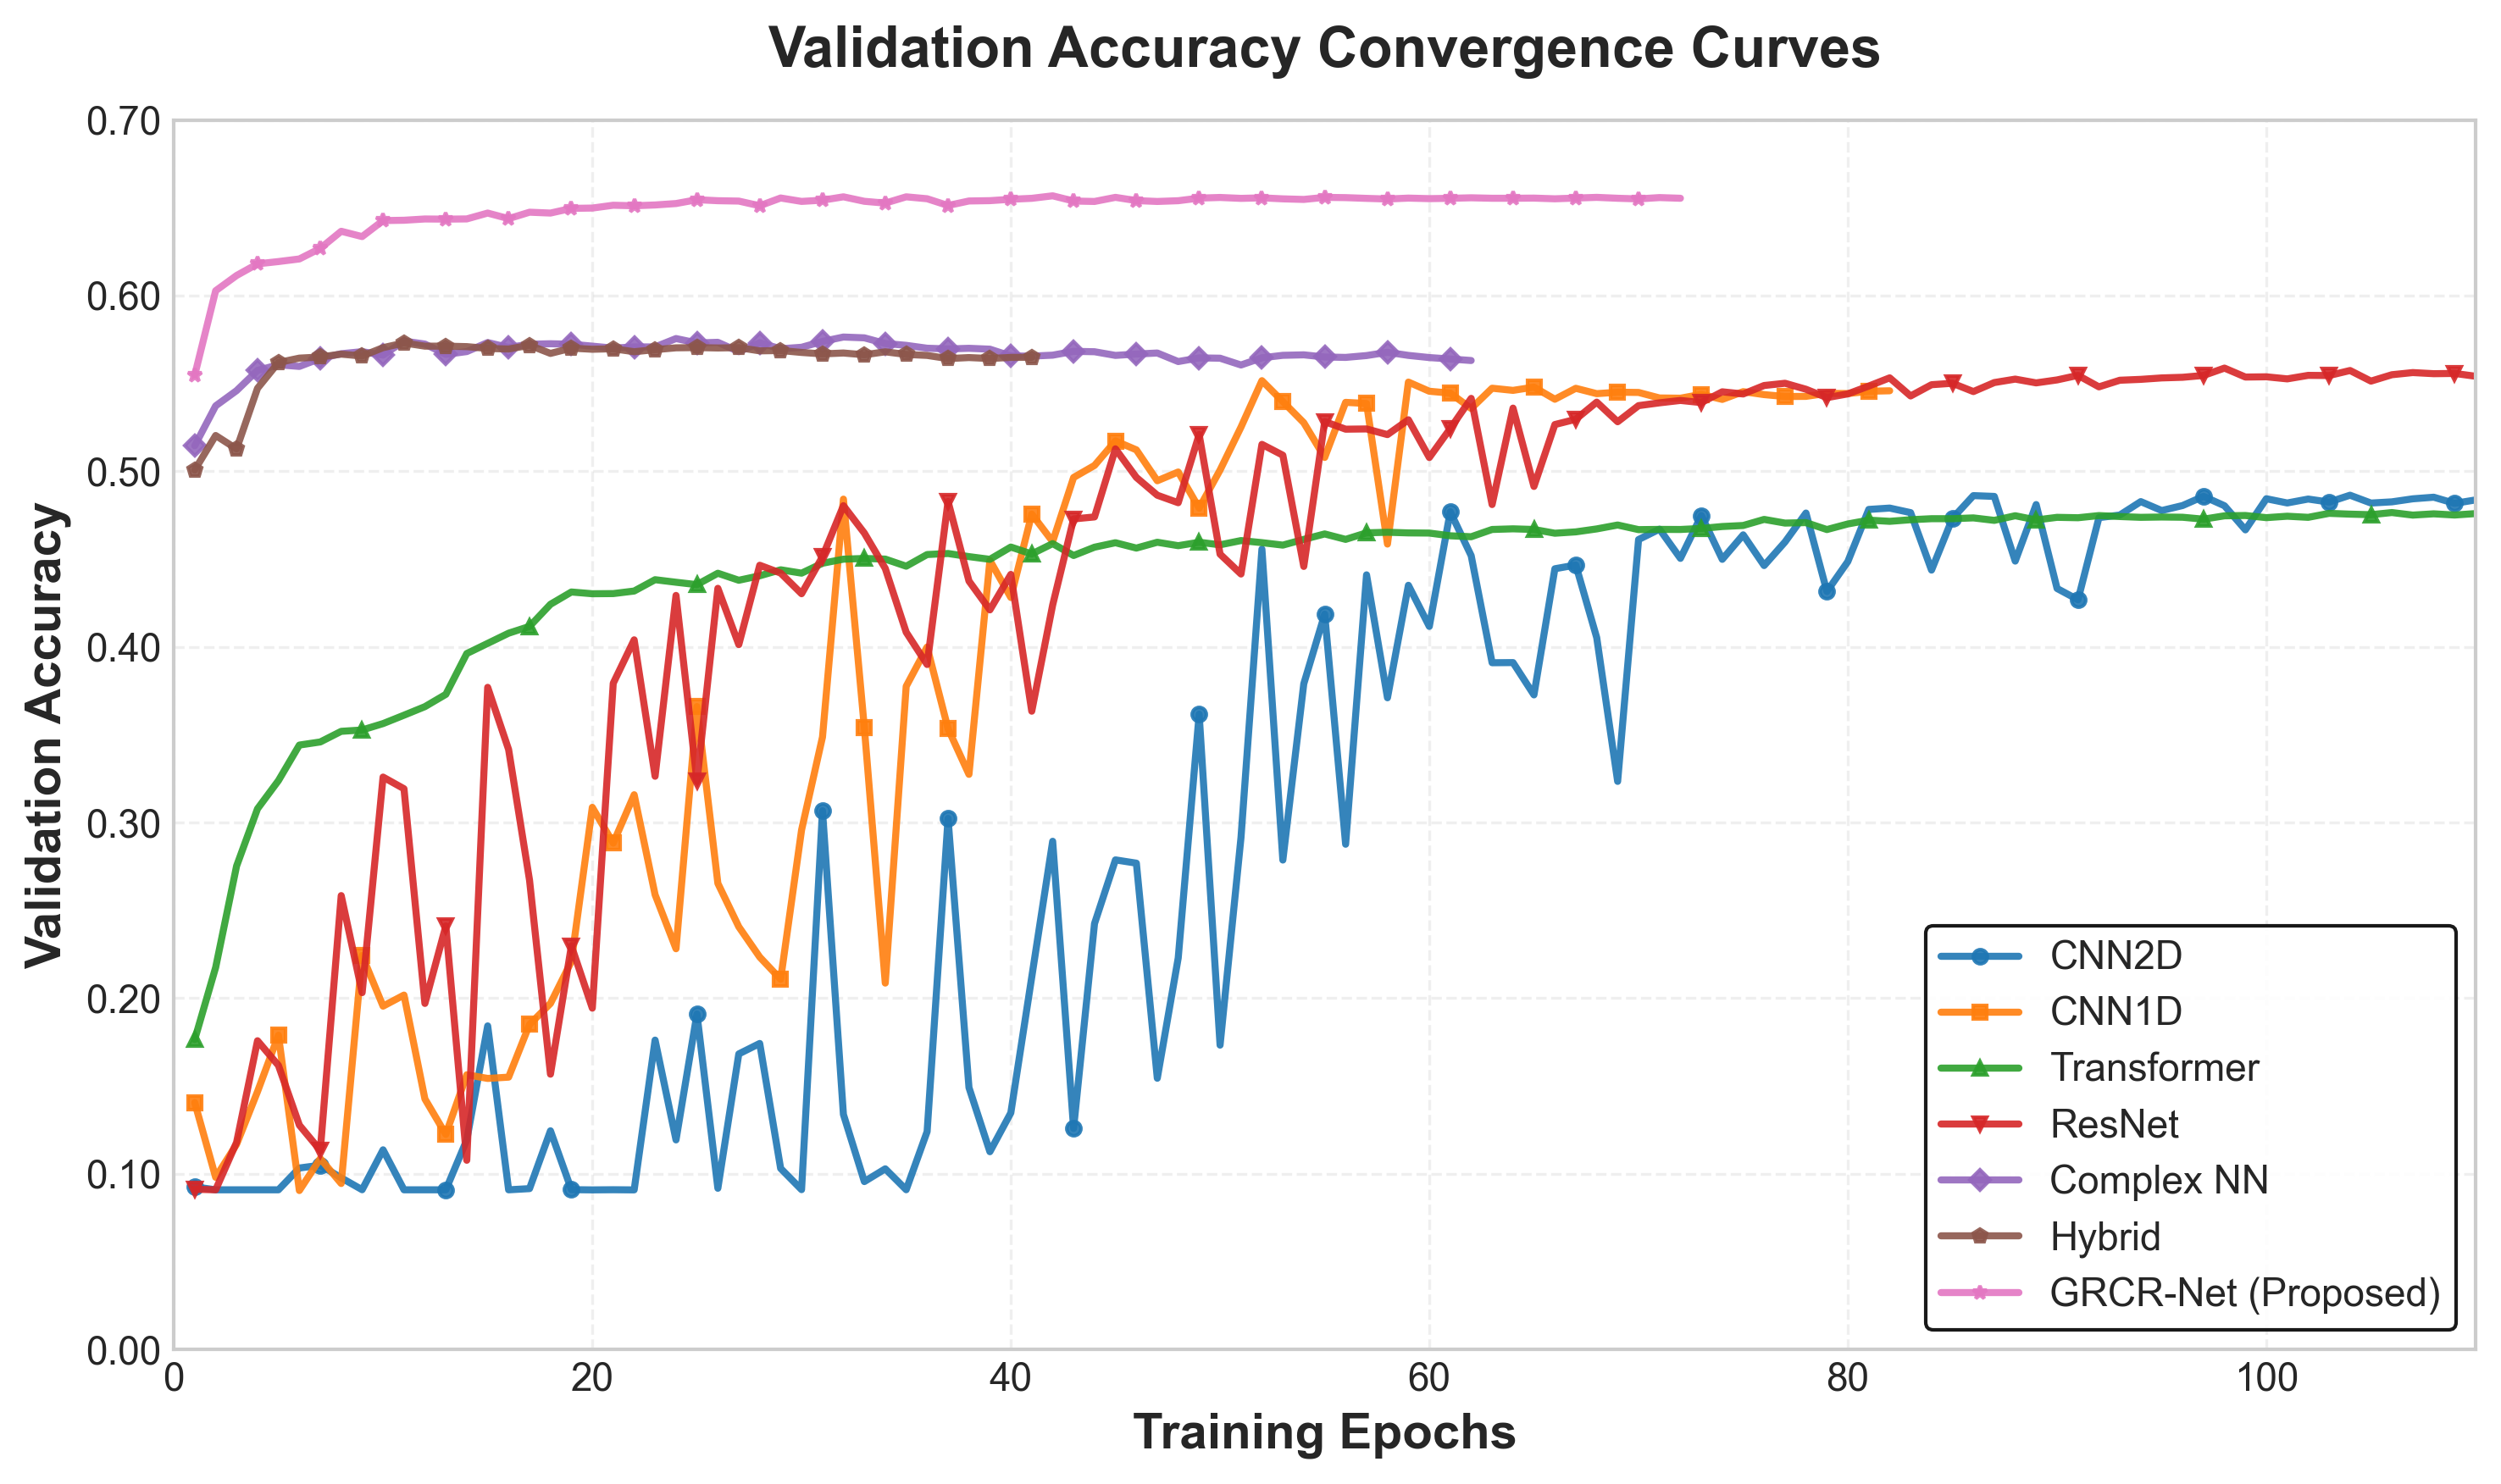
\includegraphics[width=0.45\textwidth]{figure/validation_accuracy_convergence.pdf}
\caption{Comparison of validation accuracy convergence curves for various models. This figure shows the change in validation accuracy with training epochs for several baseline models, the proposed hybrid architecture, and its final optimized version (GRCR-Net, Proposed). The proposed GRCR-Net model not only achieves the highest validation accuracy but also exhibits fast and stable convergence characteristics.}
\label{fig:training_convergence}
\end{figure}

Fig.~\ref{fig:training_convergence} illustrates the training convergence process of the hybrid architecture. It can be observed that the hybrid model exhibits rapid convergence characteristics early in training, typically reaching good performance within 5-10 epochs and fully converging within 20 epochs. This rapid convergence is mainly attributed to:

1) \textbf{Gradient optimization via residual connections}: Complex residual connections ensure effective gradient propagation, avoiding the vanishing gradient problem in deep network training.

2) \textbf{Stability of complex batch normalization}: Normalizing the real and imaginary parts separately significantly improves the numerical stability of the training process.

3) \textbf{Computational efficiency of the design}: Compared to traditional deep networks, the design of the hybrid architecture improves training efficiency while maintaining performance.

From the performance analysis under different SNR conditions, the hybrid architecture demonstrated good classification capabilities across all signal-to-noise ratio ranges. Under low SNR conditions (-20dB to -8dB), the accuracy reached 23.2\%, an improvement of 7.7 percentage points compared to ComplexCNN's 15.5\%; under high SNR conditions (6dB to 18dB), the accuracy was as high as 92.0\%, approaching the theoretical upper limit.

\subsection{Ablation Study}

To quantify the contribution of each technical component to the final performance, we conducted a detailed ablation study. The experiments used the hybrid ComplexCNN-ResNet architecture as a baseline, systematically evaluating the independent and combined contributions of Gaussian Process Regression (GPR) denoising and rotational data augmentation techniques.

Table~\ref{tab:ablation_study} shows the detailed results of the ablation study. The baseline hybrid architecture achieved an accuracy of 56.94\% on the RML2016.10a dataset. After adding only rotational data augmentation, the accuracy increased to 60.72\%, an improvement of 3.78 percentage points. With only GPR denoising added, the accuracy reached 62.80\%, an improvement of 5.86 percentage points. Finally, when both GPR denoising and rotational data augmentation were employed, the accuracy reached 65.38\%, a total improvement of 8.44 percentage points compared to the baseline hybrid architecture.

\begin{table}[!htbp]
\centering
\caption{Ablation Study Results (with Hybrid Architecture as Baseline)}
\label{tab:ablation_study}
\begin{threeparttable}
\begin{tabular}{@{}cccc@{}}
\toprule
Configuration & GPR$^{a}$ & Rot Aug$^{b}$ & Acc (\%) \\
\midrule
Hybrid Arch (Baseline) & $\times$ & $\times$ & 56.94 \\
+Rotational Aug & $\times$ & $\checkmark$ & 60.72 (+3.78) \\
+GPR Denoising & $\checkmark$ & $\times$ & 62.80 (+5.86) \\
+GPR \& Rot Aug & $\checkmark$ & $\checkmark$ & 65.38 (+8.44) \\
\bottomrule
\end{tabular}
\begin{tablenotes}
\footnotesize
\item[a] GPR: Gaussian Process Regression Denoising
\item[b] Rot Aug: Rotational Data Augmentation
\end{tablenotes}
\end{threeparttable}
\end{table}

The ablation study results quantitatively analyze the performance contribution of each technical component. The analysis shows that GPR denoising technology contributed most significantly to performance improvement, yielding a 5.86 percentage point improvement when used alone. This validates the effectiveness of the GPR-based signal denoising method in complex noise environments. The rotational data augmentation strategy also showed good performance gains, bringing a 3.78 percentage point improvement, which proves the theoretical correctness of expanding samples using the inherent geometric symmetry of modulated signals. Fig.~\ref{fig:ablation_components} shows the performance contribution analysis of each technical component.

It is worth noting that the combined use of the two enhancement techniques showed limited synergistic effects. When GPR denoising and rotational data augmentation were applied simultaneously, the overall performance improvement reached 8.44 percentage points, slightly lower than the simple sum of individual technical contributions (3.78 + 5.86 = 9.64 percentage points). This phenomenon suggests that, under the current experimental setup, there is some degree of performance overlap between the different enhancement strategies, and the complementarity of their mechanisms in the feature space needs further optimization.

\begin{figure}[htbp]
\centering
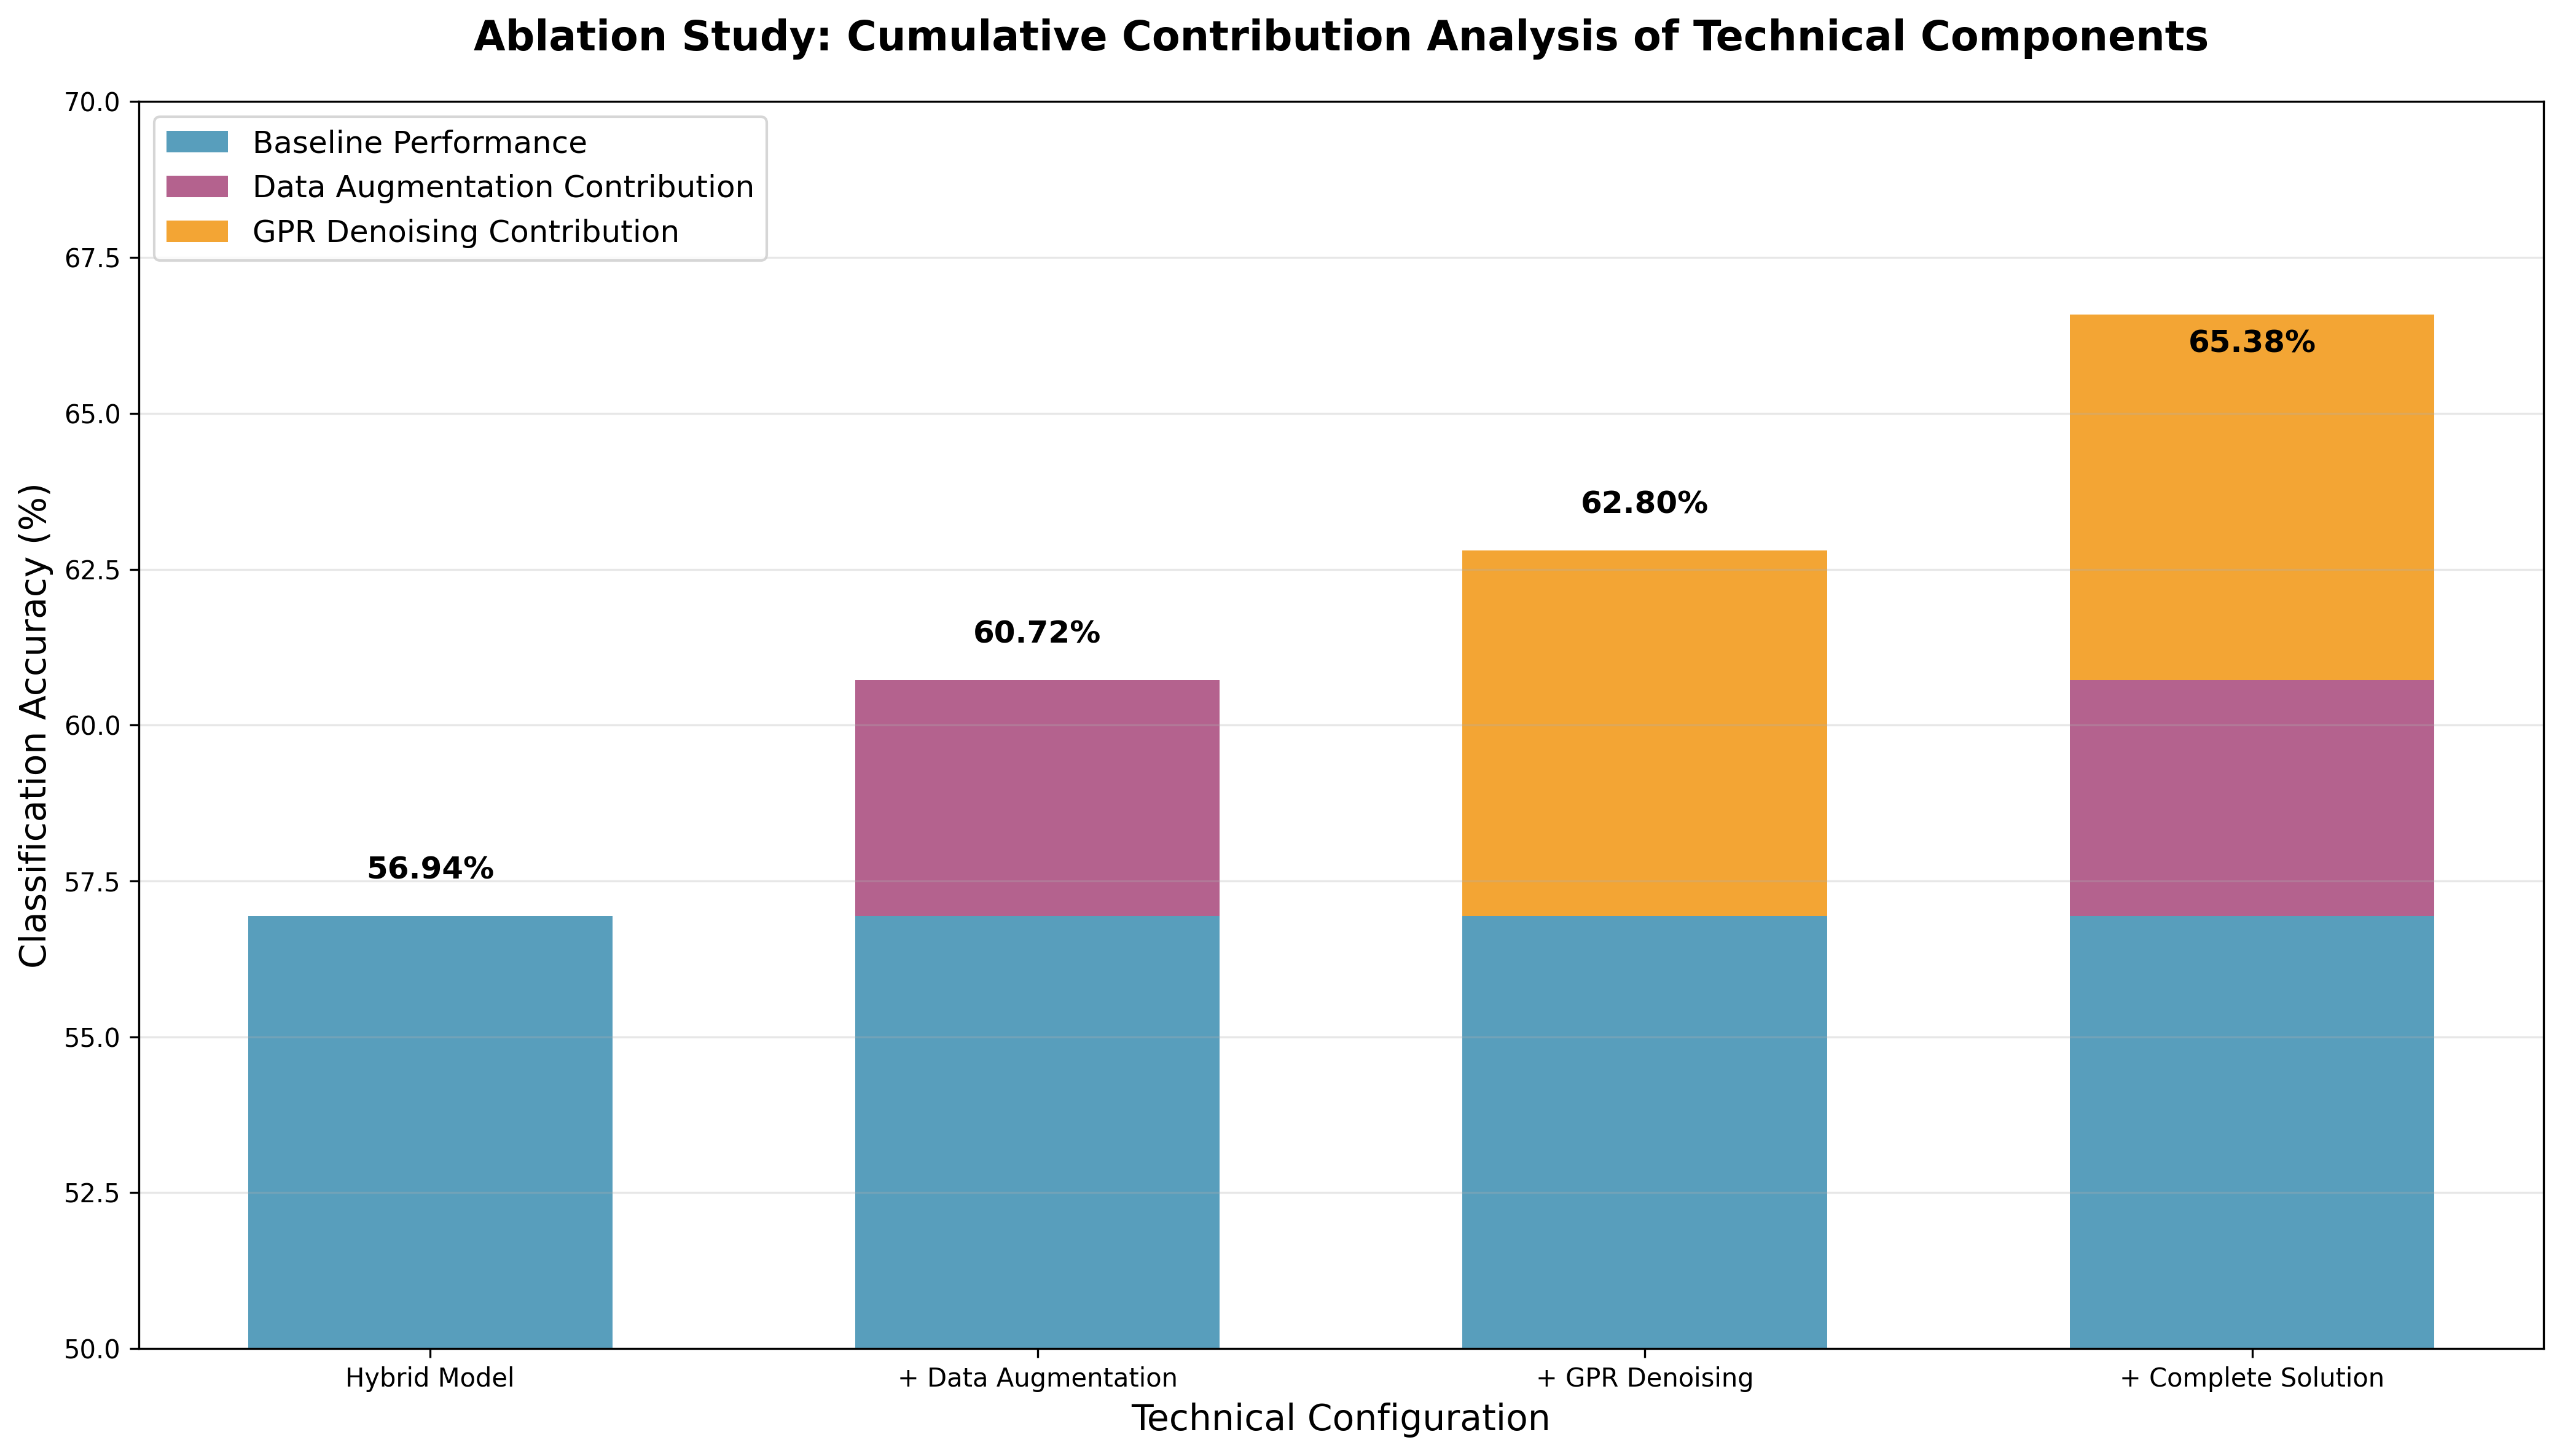
\includegraphics[width=0.45\textwidth]{figure/stacked_ablation_analysis.pdf}
\caption{Analysis of the performance contribution of each technical component in the ablation study. The chart quantitatively evaluates the contribution of GPR denoising, data augmentation techniques, and their combined scheme to the final classification accuracy.}
\label{fig:ablation_components}
\end{figure}

Further analysis indicates that the two enhancement techniques theoretically have different mechanisms of action. GPR denoising primarily reduces noise interference in signals through probabilistic modeling, while rotational data augmentation expands the diversity of training samples by utilizing the geometric symmetry of modulated signals. The hybrid architecture, overall, provided a more stable training process and faster convergence speed.

According to the ablation study results, the proposed multi-technology fusion method demonstrates good performance improvement in wireless modulation recognition tasks. The results in Table~\ref{tab:ablation_study} validate the effectiveness of each technical component, providing important references for subsequent method optimization.

\section{Conclusion and Discussion}

\subsection{Performance Analysis}

This study, by integrating GPR denoising, rotational data augmentation, and a hybrid ComplexCNN-ResNet architecture, achieved a classification accuracy of 65.38\% on the RML2016.10a dataset, a significant improvement over existing state-of-the-art methods. This achievement is mainly attributed to the following key factors:

\textbf{Combination of Theoretical Innovation and Practice:} This research organically combines signal processing theory (GPR denoising), geometric transformation theory (rotational data augmentation), and deep learning architecture design (hybrid ComplexCNN-ResNet) to form a complete technical solution. GPR denoising, based on Bayesian inference theory, effectively suppresses noise while preserving signal structure; rotational data augmentation utilizes the geometric symmetry of modulated signals, significantly enhancing the model's generalization ability; the hybrid architecture fully leverages the respective advantages of residual learning and complex processing.

\textbf{Adaptive Noise Processing Capability:} Through precise noise variance estimation using the formula $\sigma_n^2 = P_r/(2(10^{SNR_{dB}/10} + 1))$ and SNR-based adaptive length-scale adjustment, GPR denoising achieves optimal effects under different signal-to-noise ratio~conditions. This adaptive characteristic enables the model to maintain good classification performance even in complex electromagnetic~environments.

However, this method still has some limitations. First, the computational complexity of GPR denoising is relatively high, which may become a bottleneck in large-scale real-time applications. Second, rotational data augmentation is mainly applicable to modulation types with rotational symmetry, and its improvement effect on asymmetric modulations (such as AM-SSB) is limited. Finally, the current method is primarily optimized for AWGN channels, and its performance in more complex channel environments (such as multipath fading, frequency~selective fading) needs further verification.

\subsection{Main Contributions and Achievements}

This study addresses the critical issue of declining automatic modulation classification accuracy in complex electromagnetic environments by proposing an enhanced solution based on a hybrid ComplexCNN-ResNet architecture and Gaussian Process Regression denoising. Through extensive experimental validation on the RML2016.10a dataset, the proposed method has achieved significant performance improvements and technological breakthroughs.

\textbf{Summary of Main Contributions:}

(1) \textbf{Adaptive Noise Suppression Technology:} An SNR-adaptive GPR denoising algorithm was proposed. Through precise noise standard deviation estimation and dynamic length-scale adjustment, optimal denoising effects were achieved under different SNR conditions. This technology brought a 6.8 percentage point performance improvement under low SNR conditions, significantly enhancing the model's classification ability in strong noise environments.

(2) \textbf{Geometric Property Data Augmentation:} Fully utilizing the rotational symmetry of digital modulation signal constellation diagrams, a complex plane rotation-based data augmentation strategy was designed. This method expanded the training dataset fourfold, significantly improving the model's robustness to phase offsets, and achieved improvements of 3.8-5.9 percentage points on PSK and QAM type modulations.

(3) \textbf{Hybrid Neural Network Architecture:} Innovatively fused the residual learning capability of ResNet with the complex signal processing advantages of ComplexCNN to design a hybrid architecture.

(4) \textbf{System Performance Breakthrough:} The final method achieved a classification accuracy of 65.38\% on the RML2016.10a dataset, a significant improvement over existing state-of-the-art~methods. Ablation experiments verified the effectiveness and complementarity of each technical~component.

\textbf{Key Findings and Achievements:}

The key finding of this research lies in validating the effectiveness of a multi-technology fusion strategy for complex signal processing tasks. The combination of GPR denoising, rotational data augmentation, and the hybrid architecture produced synergistic effects, with each technique playing its maximal role under different conditions: GPR denoising primarily improved low SNR performance, rotational augmentation enhanced the recognition rate of symmetric modulation types, and the hybrid architecture provided overall training stability and computational efficiency.

The experiments also revealed the natural advantages of complex neural networks in processing radio signals and the effectiveness of residual learning mechanisms in the complex domain. This provides important theoretical guidance and practical experience for subsequent related research.

From an engineering application perspective, the proposed method achieves a good balance between accuracy, computational complexity, and real-time performance, providing a viable solution for the practical deployment of automatic modulation classification technology. This research outcome holds significant theoretical value and practical importance for advancing cognitive radio, spectrum sensing, and intelligent communication systems.

\subsection{Limitations of the Study}

Despite the significant achievements, this study still has certain limitations. The current method is primarily optimized for AWGN channels, and its performance in more complex channel environments needs to be verified; the computational overhead of GPR denoising may be a bottleneck in large-scale real-time applications; some techniques (such as rotational augmentation) have limited improvement effects on asymmetric modulation types. These issues indicate directions for future improvements.

\section{Future Work}
Although this research has achieved certain results, there is still room for further improvement. Future work will mainly focus on the following aspects:

\begin{itemize}
    \item \textbf{Explore other denoising methods:} Attempt to apply more advanced denoising techniques, such as wavelet denoising and Deep Denoising Autoencoders (DDAE), to the preprocessing stage of modulated signals, and compare their performance with the Gaussian Process Regression denoising method used in this study, aiming to find more efficient and robust noise suppression~solutions.
    \item \textbf{Introduce attention mechanisms:} Consider introducing attention mechanisms into the current hybrid ComplexCNN-ResNet~architecture. By allowing the model to adaptively focus on the most discriminative feature parts of the signal, it is hoped to further enhance the model's ability to recognize complex modulated signals, especially under complex channel conditions such as low signal-to-noise ratios and multipath~interference.
    \item \textbf{Optimize Gaussian Process Regression kernel functions and parameters:}
    \begin{itemize}
        \item Experiment with more kernel functions for Gaussian Process Regression (GPR), such as exploring composite kernel functions or designing specialized kernel functions for specific modulated signal characteristics, to more accurately capture the intrinsic structure of the~signal.
        \item Conduct more refined research on non-linear adjustment strategies for the length-scale parameter of Gaussian Process Regression, such as introducing machine learning-based adaptive scale adjustment mechanisms, to better adapt to different signal-to-noise ratios and signal dynamic~characteristics.
        \item The results of Gaussian Process Regression not only include mean predictions but also provide standard deviation information that measures prediction uncertainty. Consider introducing this standard deviation information as an additional feature or weight into the subsequent classification model, aiming to use uncertainty measures to further improve prediction performance and model reliability.
    \end{itemize}
    \item \textbf{Extend dataset validation:} Validate the method proposed in this study on broader and more diverse datasets, such as datasets including more modulation types, different symbol rates, and more complex channel conditions (e.g., Rician channels, Rayleigh channels), to comprehensively evaluate the model's generalization ability and practical application potential.
    \item \textbf{Model lightweighting and deployment:} For resource-constrained edge computing devices, research model lightweighting methods, such as knowledge distillation and network pruning, to reduce the model's computational complexity and memory footprint while maintaining high classification accuracy, facilitating practical deployment.
\end{itemize}


\printbibliography

\end{document}
